\section{Introduction}

This document describes a set of recommendations for the initial implementation of the Vera C. Rubin Observatory's Legacy Survey of Space and Time (LSST) observing strategy. These recommendations were produced by Rubin Observatory's Survey Cadence Optimization Committee (SCOC) as ``Phase 2'' recommendations and are intended as guidance to Rubin Observatory's Director to implement the LSST observations. It should be noted, and it is discussed in detail in this document, that aspects of the observing strategy are still under refinement, and that the observing strategy should be continuously reevaluated during operation to ensure it continues to maximize the scientific throughput of the survey.

The present document assumes the reader has a basic familiarity with Rubin Observatory, the LSST, and the process of converging to an observing strategy that will achieve the many scientific goals of the survey. The reader is referred to documents including \citealt{LPM-17}, \citealt{PSTN-051}, \citealt{PSTN-053}, and \citet{2022ApJS..258....1B}, among others, to acquire the relevant background information. 

The SCOC is a standing committee instituted in 2018 as an advisory body to Rubin Observatory's Director of Operations with the charge to:
\begin{itemize}
\item Recommend an initial survey strategy for the Rubin Legacy Survey of Space and Time, which includes defining:
\begin{itemize}
\item Footprint to be observed in the Wide Fast Deep Survey (hereafter, WFD),
\item Footprint to be observed in ``special regions'' outside of the WFD,
\item Cadence for observing the WFD,
\item Cadence for observing special regions and time to be spent on special regions,
\item Filter balance over the WFD,
\item Filter balance over the rest of the footprint,
\item Selection of the Deep Drilling Fields (hereafter DDFs),
\item Time to be spent on the DDFs,
\item Cadence for observing DDFs,
\item Propose evaluation mechanisms for adoption and prioritization of community proposals for surveys beyond the WFD.
\end{itemize}
\item Develop an ``Early Science'' plan.
\item Review the survey strategy during Operations on a regular basis and recommend adjustments.
\end{itemize}

The detailed charge of the SCOC and its membership can be found at \url{https://www.lsst.org/content/charge-survey-cadence-optimization-committee-scoc}. In reference to the development of an early science plan, we note that the first year of the LSST is likely to require a different strategy implementation than the rest of the survey and detail of the observing strategy in year 1 remain be defined by the SCOC and Rubin Operations team (see \citealt{rtn-011} and \autoref{q:Early}).

Over the past decade, Rubin Observatory has engaged the community in the design of the details of Rubin LSST, beyond the broad constraints imposed by the four core science deliverables of Rubin as described in the Science Requirements Document by \citet[][hereafter SRD]{LPM-17}, in a process which is described in \citet{2022ApJS..258....1B}. 

After its formation, the SCOC solicited %\footnote{Through a call available at \url{https://docs.google.com/document/d/1SYKsJkNVIGE1t5vbZ_L0qLLsV7UHeraXNVZ22-xFk4c}.}
and reviewed 39 Cadence Notes\footnote{\label{fn:cnotes}Available at \url{https://www.lsst.org/content/survey-cadence-notes-2021}.} proposing changes and enhancements to the then current plan for LSST, and a large number of LSST simulations (created through the \opsim\ framework as described in \citealt[][hereafter PSTN-051]{PSTN-051}). Collecting community feedback and metrics, the SCOC ``Phase 1'' process culminated in the recommendations released in \citetalias[or MAF][]{PSTN-053} and hundreds of v2.X simulations produced by the Survey Strategy team of Rubin Observatory that reflect these recommendations and vary the parameters yet to be finalized. 
Through December 2021 and beyond, the Survey Strategy Team, as charged by the SCOC, has also supported the community through the process of producing and integrating science-driven evaluations of the simulations into the \texttt{rubin\_sim} software\footnote{\url{https://github.com/lsst/rubin_sim}.}. These simulations and science-driven metrics produced within the Metric Analysis Framework \citep{2014SPIE.9149E..0BJ} or \texttt{MAF},  constitute a core input utilized by the SCOC, together with feedback received from the community in a variety of ways, to produce the Phase 2 recommendations described below. 




\subsection{Brief Synopsis of Phase 2 recommendations}\label{sec:shortrec}

While additional work is needed to finalize a plan for the initial LSST survey strategy (see \autoref{sec:refinements} for a summary of forthcoming refinements), the set of recommendations we present here narrows the parameter space of the possible LSST strategies substantially. Based on evaluations of possible observing strategies demonstrated in simulations from \opsim\ v2.0 through v2.99 (see \autoref{ssec:process}), the SCOC is recommending a survey strategy with the following characteristics:



\setlength\parindent{0.7cm}
\hangindent=0.7cm A WFD low-dust region definition with limits $−70\degree \leq$ Dec $< +15\degree$ for
RA $\sim 7–18$~h and $−70\degree \leq$ Dec $<+3\degree$ for 0 $\lesssim$ RA $\lesssim$ 7~h and 18~h $\lesssim$ RA $\lesssim$  24~h,  and the addition of the Virgo cluster in the WFD survey. The current recommendation for the Galactic Plane and Bulge coverage is driven by the expert advice of the SMWLV and TVS Science Collaborations but enforces higher contiguity in space coverage to better exploit specific Rubin strengths and capabilities, and improve survey efficiency. We encourage the Galactic science community to continue to work with the SCOC to finalize the survey footprint on the Galactic sky. The fraction of time spent in each of the low-dust WFD footprint, the Galactic sky, the South Celestial Pole (SCP), and the North Ecliptic Spur (NES) remains close to the fractions recommended in Phase 1 (see \citealt{PSTN-053}, section 2), and for each of these surveys the \texttt{baseline\_v3.0} implementation is within 2\% of \texttt{baseline\_v2.0} (\autoref{q:Footprint}). 

\hangindent=0.7cm Maintaining the filter balance as was implemented in \texttt{baseline\_v2.0} for the low-dust WFD region and, tentatively, for the Galactic Plane/Bulge and other special regions. However, we  encourage members of the scientific community with specific interest and expertise in the science performed with data from the special surveys to evaluate if a modified filter balance in these regions could better support the desired science outcomes (\autoref{q:Filters}).

\hangindent=0.7cm Visit pairs are maintained with a $\sim33$ minute time gap, to be collected in different filters (the filter matches may be subject to further refinement). The SCOC recommends that the LSST cadence be designed to ensure coverage of time scales in the hours-to-one-day range generally lacking in most simulations prior to v2.99.
This can be achieved with a third nightly visit at several hours separation once every several ($\sim7$) nights and increasing the probability of visits in the following night (in one of the bands that were already observed). This strategy, when implemented jointly with rolling, provides coverage at time scales from a few to 30 hours (\autoref{q:Visits}) which would otherwise be undersampled.  

\hangindent=0.7cm Rolling, \emph{i.e.} a cadence where a portion of the sky is emphasized at a point in time, to then be de-emphasized later, is recommended on the WFD, with the sky split into two 1/2-sky regions defined by declination limits and with a 0.9 rolling weight. This recommendation is made under the assumption that sufficient uniformity in depth to support static-sky cosmology can be achieved with a software solution.  Should this not be the case, the SCOC will re-evaluate this recommendation (\autoref{q:Rolling}).

\hangindent=0.7cm That no less than 5\% of the survey, with the potential to increase this to as high as 7\%, be dedicated to observing 5 pointings as LSST Deep Drilling Fields (DDFs)\footnote{See \url{https://www.lsst.org/scientists/survey-design/ddf}.}. In the current simulations, with this time investment the DDFs will generally reach a 10-year coadded depths $\sim1.3$ magnitudes deeper in each band than the coadded depth of a WFD pointing in the same band. To select the Euclid Deep Field South as the fifth LSST DDF with a footprint that can be covered with two LSST pointings, each to be observed at 0.5 of the 10-year DDF depth;  that all DDFs be observed for 10 years and the COSMOS field be observed to full 10-year depth within the first 3 years of LSST and continue to be observed thereafter at the same rate as the other DDFs. The detailed intra-night strategy on the DDFs is still under design (\autoref{q:DDF}).

\hangindent=0.7cm The SCOC recommends that two microsurveys are scheduled  in year 1: the near-sun NEO twilight survey and, if time is
available, the Northern Strip survey. Additional microsurveys should be added in the future, when the system characteristics and survey efficiency are better assessed, and a process is recommended to receive and review refined and additional microsurvey proposals after the beginning of LSST (\autoref{q:Micro}).

\hangindent=0.7cm The SCOC recommends a Target of Opportunity (ToO) program be enabled to respond to Gravitational Waves and Multi-Messenger Astronomy triggers with a fraction of $\leq 3\%$ of dedicated survey time, with the possibility of extending it to additional types of targets in the future; a path toward a process to formulate recommendations for target selection and observing strategy details is outlined (\autoref{q:ToO}).

\hangindent=0.7cm Finally, the SCOC commits to working with the Operations team in 2023 to establish the best strategy for Early Science (see \citealt{rtn-011}). Optimizing the LSST year 1 observing schedule for early science may mean that the time  sampling will look somewhat different from that in subsequent years (\autoref{q:Early}).

\noindent The SCOC will continue to refine the recommendations presented here and work closely with Rubin Observatory's Project and Operation teams to update the recommendation with knowledge of the system as built and the outcomes of Commissioning and Science Verification.


\subsection{The process of formulating Phase 2 recommendations}\label{ssec:process}

%The current recommendations presented here constitute ``Phase 2'' of the LSST strategy optimization process and substantially narrow the parameter space of the possible LSST strategy options. 

To converge to the recommendations presented herein, the SCOC has reviewed close to 500 simulations (v2.X) and hundreds of metrics, including metrics evaluating the impact of the cadence choices on the system, compliance with the \citepalias{LPM-17}, and performance on community-contributed science goals. The simulations were released in batches starting in November 2021, and they are described in detail in a  community.lsst.org post\footnote{\url{https://community.lsst.org/} is an online forum used by Rubin for discussions and announcements. The specific post describing the v2.X simulations is \url{https://community.lsst.org/t/survey-simulations-v2-1-april-2022/6538}} and on GitHub.\footnote{\url{https://github.com/lsst-pst/survey_strategy/blob/main/fbs_2.0/SummaryInfo_v2.1.ipynb}.}

After reviewing \opsim\ v2.X, the SCOC commissioned the production of and reviewed $\sim 10$ simulations (\opsim\ version v2.99) that largely straddled the remaining survey strategy options. An initial set of four simulations were released on October 24, 2022\footnote{\url{ https://community.lsst.org/t/draft-of-v3-0-survey-strategies-v2-99/7159}.} and were presented at the Third SCOC-Science Collaborations Workshop on November 2-3, 2022.\footnote{\url{https://project.lsst.org/meetings/scoc-sc-workshop3/home}.}  Additional simulations refined the v2.99 initial set of four and implemented suggestions collected during and after the November 2022 workshop. Among those simulations, we selected the one that best represents our current recommendation as \texttt{baseline\_v3.0} (described in \autoref{sec:v3})

The detailed process of reviewing input and converging to an optimal recommendation is complex, because, in this context, ``optimal'' is difficult to define. While this process of generating survey simulations and associated metrics does provide quantitative measures of enhancement of the survey, it should be noted that the metrics are not always directly comparable, nor is the overall importance of the science they reflect an objectively measurable quantity, such that a purely numerical optimization process is not possible. The performance of the strategy on different science drivers has to be balanced in the light of (1) the output of available metrics, but also (2) expert considerations about the relative importance of the performance gain/loss for different science drivers, (3) the significance of the performance change (\emph{i.e.} the metrics are not ``standardized'' in a collective sense as they measure quantities with different units and that may not be directly comparable), and (4) how core a science goal is to the overall Rubin LSST science endeavor. At a high level, the SCOC reviews the increase/decrease in performance for a science case as compared to the earlier LSST plans, known as the ``baseline'' (in the case of the Phase 2 recommendations, comparing the \texttt{v2.0} and \texttt{v2.1} simulations with the \texttt{baseline\_v1.7}, and  the simulations that implement the current recommendations ---\texttt{v2.99} and \texttt{v3.0}--- with \texttt{baseline\_v2.X}). Generally, performance changes on metrics greater than a few percent are regarded as significant. Further refinement is beyond the current scope of the SCOC work, particularly considering the as-of-yet unknown performance of the system as built. Finally, the process of optimizing the survey is further complicated by the fact that the SCOC is provided with LSST families of simulations that aim to stretch the survey in one or another direction (\emph{e.g.}, modifying the footprint or the rolling scheme). This is typically done in isolation, but the SCOC needs to keep track of and balance the compound effects of survey changes across multiple parameters, which might significantly impact a science case even when individually they had a small effect. 

The SCOC does not only review the MAF metrics performance but also provides \emph{key interpretability} to the metrics and their performance. For this the SCOC is composed of experts in different domains, attempting to cover all science areas relevant to Rubin. It should be noted, however, that SCOC members are explicitly instructed not to view themselves as advocates of specific science areas, but rather as members exercising their best judgment on the LSST observing strategy with the goal of maximizing the \emph{overall} scientific throughput of the survey.

The SCOC has also liaised with the eight Science Collaborations (SCs) of LSST, with 1--3 members of the SCOC assigned to each SC as liaisons.\footnote{See \url{https://www.lsst.org/content/charge-survey-cadence-optimization-committee-scoc} for the full list of SCOC liaisons.} In this role, SCOC members are charged with enabling and ensuring a bidirectional communication flow between the SCOC and the SCs. 

The SCOC is committed to transparency. Communication between the SCOC and the community is made through a number of channels: via liaisons to the SCs; summaries of the SCOC goals and discussions on community.lsst.org;\footnote{See the dedicated ``Survey Strategy'' topic (\url{https://community.lsst.org/c/sci/survey-strategy/37}).} presentations of our current work and status of the recommendations at relevant meetings, including the annual Project Community Workshop (PCW); and by organizing dedicated workshops to come together with the community. Most recently the SCOC and community met in the Third SCOC Workshop on November 2-3, 2022.\footnote{\url{https://project.lsst.org/meetings/scoc-sc-workshop3/home}.} Phase 2 recommendation updates have been released in a post on community.lsst.org\footnote{\url{https://community.lsst.org/t/scoc-v2-0-and-2-1-simulations-review-timeline/6712}.} leading to the November workshop, including short summaries of the discussion as conducted in each full SCOC meeting.\footnote{Released in \url{https://community.lsst.org/t/scoc-v2-0-and-2-1-simulations-review-timeline/6712}.} Starting in November 2022, a dedicated community post is regularly updated with meeting summaries and future meetings' schedules,\footnote{\url{https://community.lsst.org/t/public-scoc-meeting-minutes/7185}.} and regular office hours have been established.\footnote{\url{https://community.lsst.org/t/scoc-office-hour/7221}.}

While we had solicited official reports in the SCOC Phase 1 deliberations (the 2019 Cadence notes,\footnote{See \autoref{fn:cnotes}.}
the SCOC decided shortly after the v2.0 simulations were made available {\it not} to solicit formal reports from the SCs and the community in the Phase 2 deliberations so as to avoid overburdening the community members. Yet several SCs shared their feedback in a number of written reports. Reports received by the SCOC in its Phase 2 deliberations include analyses of the \opsim\ via metrics relevant to a specific science-focused group, as well as  considerations not based on metrics but on expert opinions from domain scientists. All these reports are made available to the reader.\footnote{Listed in the order in which they were received, these include reports from the
SSSC (May 2022);
the TVS and SMWLV SCs (a report on Galactic science and a more specific report on microlensing), TVS SC (on exctra-galactic science), and TVS and AGN SCs (the latter four all first received in March 2022); three 
DESC reports (June 2022, October 2022, and November 2022); a report from the AGN SC (August 2022); all these reports are available on the SCOC website at \url{https://lsst.org/content/reports-scs-v2x-simulations}.} Feedback delivered to the SCOC in the form of written reports, through interactions on community.lsst.org,\footnote{Including the thread \url{https://community.lsst.org/t/scoc-v2-0-and-2-1-simulations-review-timeline/6712}.} as well as reported by the SCOC liaisons was considered and incorporated in our decision-making process. 


As discussed above, the comparison of results of the metrics, hereafter referred to as metrics or MAFs, produced by the Survey Strategy team (primarily to assess compliance with the SRD and other system requirements) and by the community constitute a quantitative ---or at least quantifiable--- feedback on LSST simulations. Three kinds of plots are generally produced to compare the performance of simulations for sets of MAFs.

\begin{itemize}

\item {\bf Radar Plots:} helpful to review and compare small numbers of simulations and small numbers of metrics. In a radar plot such as \autoref{fig:radar} each vertex corresponds to a MAF, and each simulation is indicated in a different color. By design, the reference simulation forms a ``perfect'' circle, where the performance for each MAF is =1. For a given simulation, a MAF performance that extends outward (inward) of the reference circle indicates an improvement (decrease in) performance. 

\begin{figure}[h!]
\centering
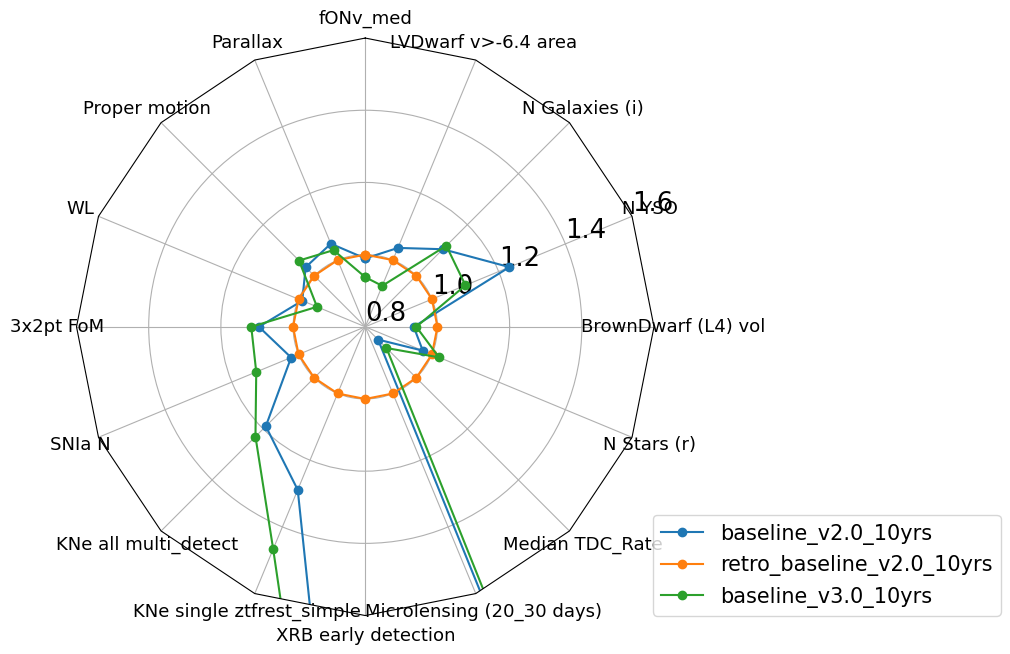
\includegraphics[height=0.4\textwidth]{figures/SCOC299radar1.png}
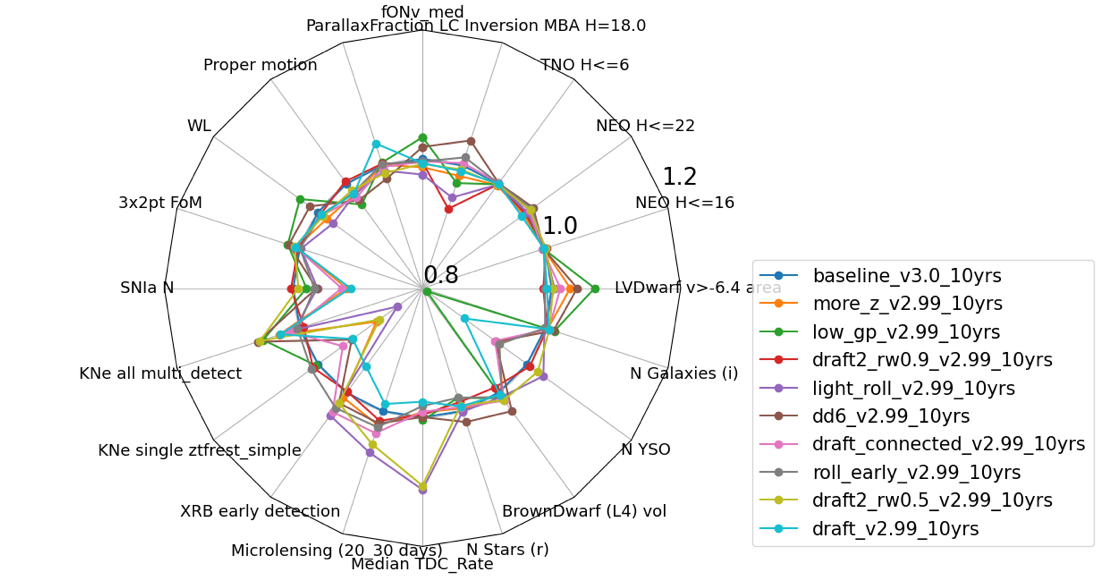
\includegraphics[height=0.4\textwidth]{figures/SCOC299radar2.png}
\caption{Radar plots comparing  \texttt{baseline\_v3.0} with earlier baseline simulations (\emph{top}) and the v2.99 simulations released starting on October 24th, 2022 with \texttt{baseline\_v3.0} (\emph{bottom}) . The majority of the metrics considered display improvements compared with earlier baseline simulations. The improvement on the ``XRB early detection'' and ``Microlensing (20\_30 days)'' metrics is $>300\%$ between \texttt{baseline\_v3.0\_10yrs} and \texttt{retro\_baseline\_v2.0\_10yrs} which reproduces baseline \texttt{baseline\_v1.7\_10yrs}, and extend outside of the range of the plot.}\label{fig:radar}
\end{figure}
\FloatBarrier

\item {\bf Heatmaps}: Larger collections of metrics and simulations are generally better visualized with heatmaps (see \autoref{fig:heatmap}), where families of simulations (as columns) and families of MAFs (as rows) can be grouped together by appropriate ordering. 


\begin{figure}[t!]
\centering
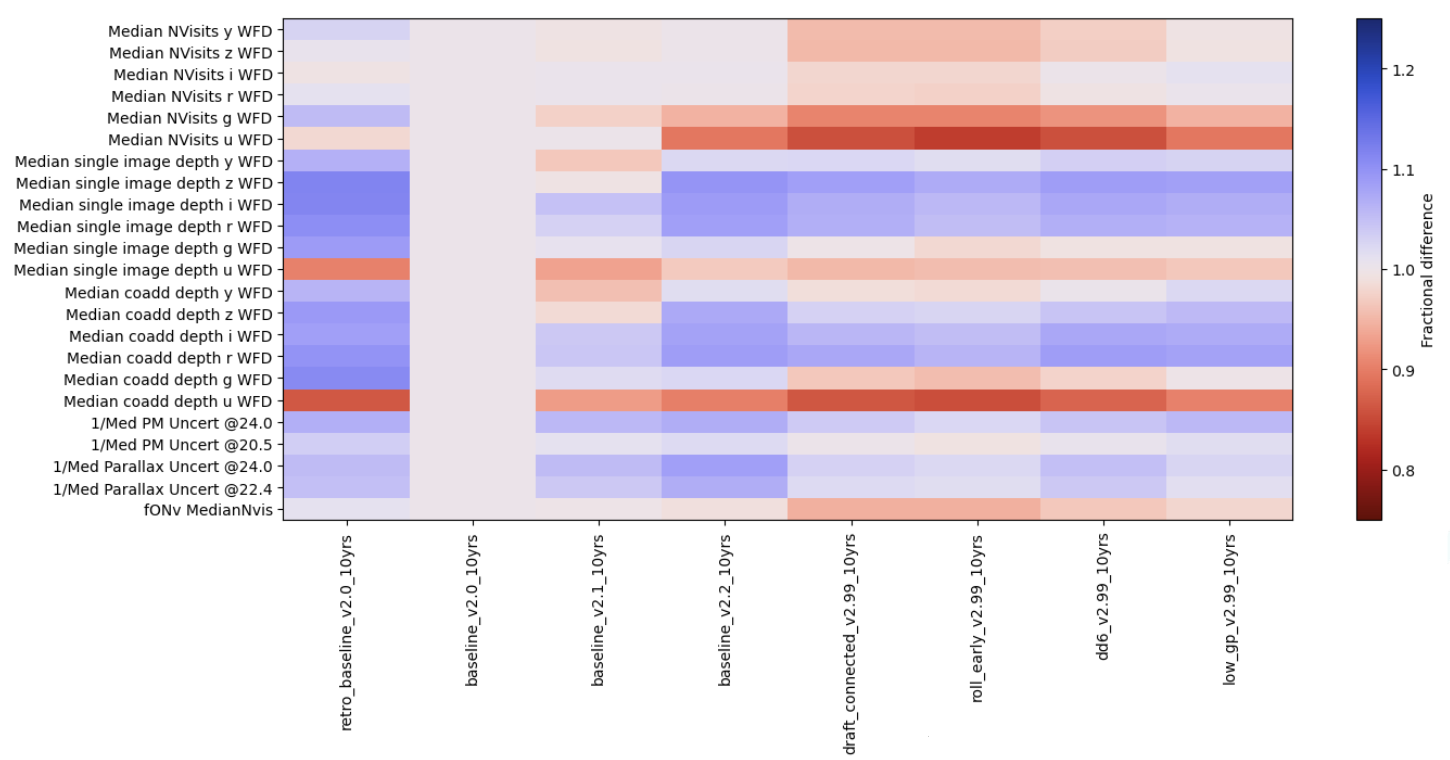
\includegraphics[width=0.8\textwidth]{figures/SCOC299heatmap1.png}
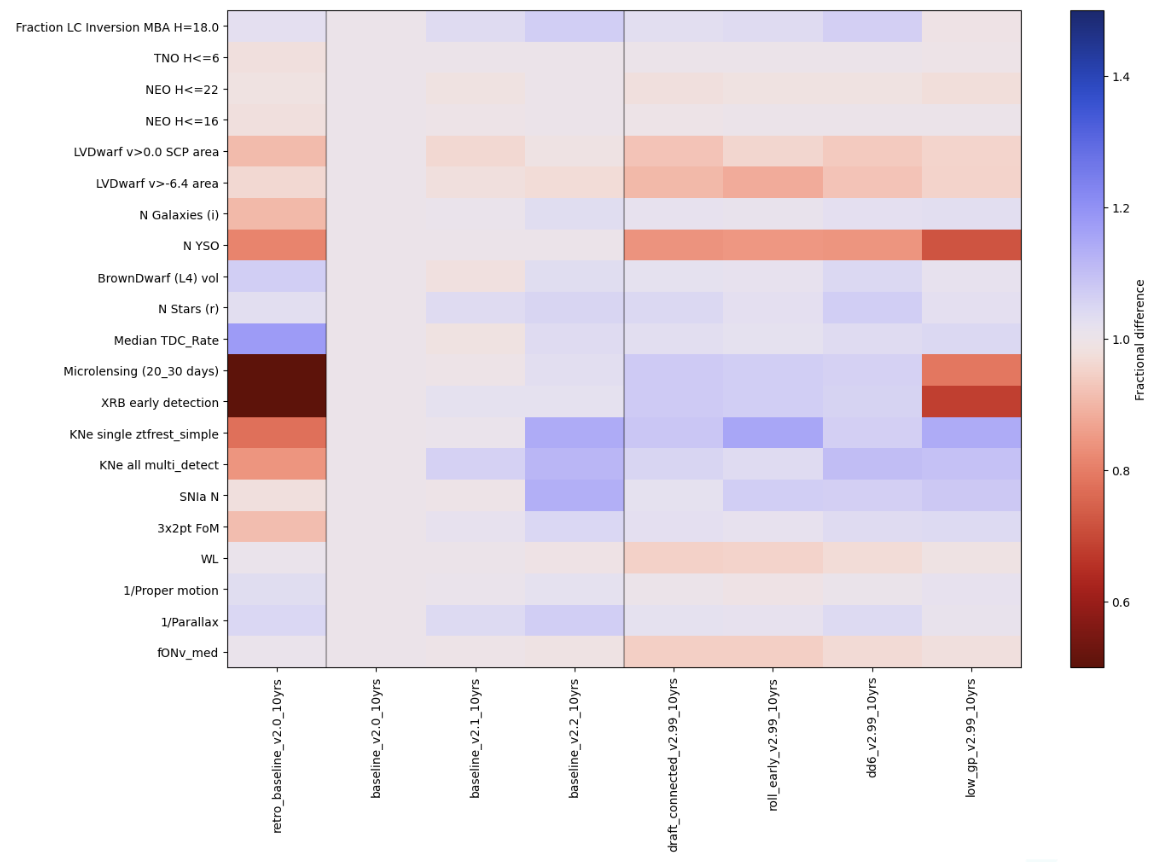
\includegraphics[width=0.8\textwidth]{figures/SCOC299heatmap2.png}
\caption{Heat maps comparing the first four v2.99 simulations (released on October 24th, 2022)  with earlier baselines for a selection of system metrics (\emph{top}) and science metrics contributed by the community (\emph{bottom}). Blue blocks indicate improvements compared to a reference simulation (here \texttt{baseline\_v2.0\_10yrs}), and red ones indicate performance loss. The increase or drop of a series of MAFs in adjacent rows may indicate a systemic problem. For example, the SCOC noticed and investigated the decrease in Galactic and Local Volume performance as measured by the number of dwarf galaxies and Young Stellar Objects (YSO) with the help of the SMWLV SC and TVS SC.}
\label{fig:heatmap}
\end{figure}
\FloatBarrier


\item {\bf Line plots}: 
While heatmaps provide a synoptic view, the amount of gain/loss is not obviously quantifiable via the color intensity. Line plots are useful to inspect small numbers of (typically related) MAFs and provide quantifiable significance of a gain/loss (see \autoref{fig:lineplot}). 


\end{itemize}
\begin{figure}[h!]
\centering
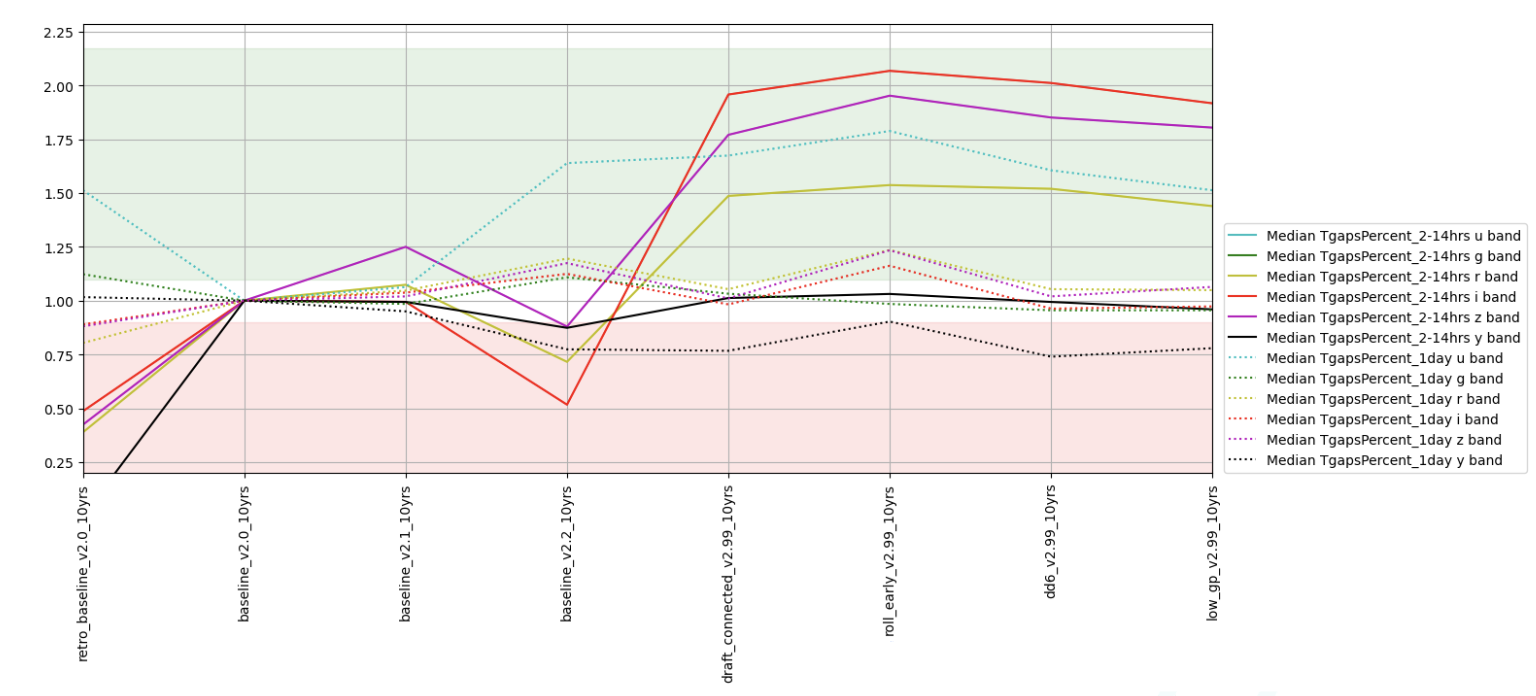
\includegraphics[width=0.99\textwidth]{figures/SCOC299lines.png}
\caption{A line plot showing the performance of metrics measuring intra-night cadence for the same simulations used in \autoref{fig:heatmap}: each MAF measures coverage on specific time scales. All values are to be compared with 1, the performance of a reference simulation (here \texttt{baseline\v2.0\_10yrs}). The shaded areas indicate potentially significant performance changes, generally set to a $>5\%$ performance difference. The SCOC notes a generally improved performance for nearly all the v2.99 Time Gap metrics, with performance gains as high as 100\% in some cases.}
\label{fig:lineplot}
\end{figure}

\FloatBarrier
The survey strategy team makes these visualizations available via jupyter notebooks organized by simulation family, MAF family (including notebooks specifically designed for an interest group or SC), and SCOC question (see below). All these notebooks are available on GitHub.\footnote{\url{https://github.com/lsst-pst/survey_strategy}.}



\subsection{Open questions addressed in Phase 2}\label{sec:synopsis}

The SCOC has organized its Phase 2 deliberation around eight topics (posted on community.lsst.org\footnote{\url{https://community.lsst.org/t/scoc-v2-0-and-2-1-simulations-review-timeline/6712} and listed at the end of this section.} in June 2021). Many of these topics came from questions that were addressed to some extent in Phase 1 but needed further study. The open questions and remaining SCOC tasks identified in earlier reports \citepalias{PSTN-051, PSTN-053} were systematically explored in the \texttt{v2.0}, \texttt{v2.1}, and \texttt{v2.2} series of \opsim\ LSST simulations\footnote{The simulations were described in \url{https://github.com/lsst-pst/survey_strategy/blob/main/fbs_2.0/SummaryInfo_v2.1.ipynb} and on community.lsst.org \url{https://community.lsst.org/t/survey-simulations-v2-1-april-2022/6538}.} and include:

%Here we report the questions considered within each topic and the information and deliberations that led to the SCOC recommendations encapsulated in the \texttt{v2.99} and \texttt{baseline\_v3.0} simulations are described in detail in the next section.

\begin{itemize}
\item Establish final survey footprint definitions (\emph{e.g.}, the exact Declination and dust extinction limits for the WFD region, the exact definition of the Galactic bulge region),
\item Decide which sets of filters should be used in sets of visits,
\item Decide the exposure duration and the number of visits in the $u$ band,
\item Optimize further the rolling cadence implementation,
\item Optimize further the DDF cadences.

\end{itemize}

The members of the SCOC further refined the scope of each question and split into eight overlapping subgroups to review the Rubin- and community-contributed metrics relevant to each topic, jointly with community feedback on the simulations. 
The goal of these subgroups was to formulate an initial recommendation to be presented to, reviewed by, and agreed upon by the whole SCOC. Subgroup presentations were distributed over the months of June through August 2022, with the majority of the subcommittee presenting and leading discussions on their recommendations ahead of the August 2022 PCW, where these preliminary recommendations were presented.\footnote{\url{https://project.lsst.org/meetings/rubin2022/agenda/survey-strategy-i}.} Further refinement of the full SCOC deliberations and further review of the recommendations resumed in mid-September 2022.

The eight subcommittees of the SCOC  and the topics they were tasked to address are:
\begin{enumerate}
\item{Early Science} (\autoref{q:Early})

\item{Footprint} (\autoref{q:Footprint})

\item{Filter Distribution} (\autoref{q:Filters})

\item{Nightly Visits pairs and triplets} (\autoref{q:Visits})

\item{Rolling Cadence} (\autoref{q:Rolling})

\item{DDF Strategy} (\autoref{q:DDF})


\item{Microsurveys} (\autoref{q:Micro})

\item{Time allocation for ToO} (\autoref{q:ToO})

\end{enumerate}

In the following section (\autoref{sec:rec}) we describe in detail the deliberation process for each of these eight topics and the associated SCOC Phase 2 recommendation. In \autoref{sec:v3} we describe the \texttt{baseline\_v3.0} simulation that implements our current recommendations. In \autoref{sec:refinements} we highlight the elements of the current recommendation that need further refinement.

%\input{v2.99_sims.tex}
\clearpage

\section{SCOC recommendations by topic}\label{sec:rec}
The following eight sections describe in detail the recommendation for each of the eight topics outlined in \autoref{sec:synopsis} and the motivations for the given recommendation. Sections of text in bold font include a summary of the recommendation, while sections of text in italic font indicate elements of the recommendation that require further study. 


\subsection{Early Science Options}\label{q:Early}
Early science recommendations include and overlap with recommendations on prioritization of sky coverage and survey-specific choices that may be adopted in year 1, when for the most part the surveyed sky will not have templates or will have substandard templates, leading to the first data release that will process the initial six months of LSST data. 

While this recommendation is within the purview of the SCOC, producing a meaningful and informed recommendation that can be implemented effectively requires close interaction with the Commissioning and Operation teams of Rubin LSST (see also \citealt{rtn-011}).

As such, we defer a  recommendation on early science to 2023, during which time the SCOC will formulate a detailed plan for interaction with the Operations team. At this stage, we see benefits in implementing a survey strategy that is specific to year 1 that allows for optimal generation of templates (for example trading more filters for less sky area or vice versa) so that alerts can be released before the first data release. The details of the strategies that optimize early science while also ensuring high throughput for the survey as a whole can only be finalized through interaction between the SCOC and Rubin Operations team. 

%\clearpage

\subsection{Footprint Refinements}\label{q:Footprint} 

The most impactful recommendation from Phase 1 was a substantial revision of the survey footprint. The recommended footprint, implemented in \texttt{baseline\_v2.0}, included a $\sim10\%$ area increase extending the WFD into low dust extinctions regions for extragalactic science and extended WFD-level coverage into high priority regions for Galactic science --- the Galactic Bulge and the Magellanic Clouds --- while removing high dust extinction Galactic Plane sky outside the Galactic Bulge from the WFD. A mini-survey area (a few 100's visits) was added to maintain some coverage of these parts of the sky. As a result of these changes, the overall area included in the survey was expanded and the number of visits per pointing dropped closer to the expected survey ``design'' values of 825 visits per pointing (see \citeds{LPM-17}) instead of the previous 900+ visits per pointing). See \citeds{PSTN-053} Q1 \& 2 for details. 

The questions left open after the Phase 1 recommendations on the survey footprint were: 

\begin{enumerate}
\item What should the exact declination and/or dust extinction limits for the WFD region be? Should the Virgo cluster be added to the WFD?
\item What should the definition of the Galactic bulge region be? 
\item What fraction of time should be spent observing the Galactic Plane?
\item What fraction of time should be spent observing the NES?
\item What fraction of time should be spent covering the SCP?
\item What fraction of time should be spent on pencil beam surveys?
\end{enumerate}

\subsubsection{SCOC recommendations: executive summary}\label{rec:footprint_es}

 The SCOC reviewed all community-contributed reports and evaluated the impact of footprint changes on metrics contributed by the Survey Strategy team and by the community. The impact of footprint choices on many relevant metrics is shown in notebooks prepared by the Survey Strategy team.\footnote{Including \url{https://github.com/lsst-pst/survey_strategy/blob/main/fbs_2.0/SkyCoverage.ipynb} and \url{https://github.com/lsst-pst/survey_strategy/blob/main/fbs_2.0/Rolling\%20Cadence.ipynb}.}

{\bf The SCOC provides here a recommendation for the definition of the extragalactic footprint, NES, and SCP (see points 1, 4, and 5 below). The SCOC has finalized a recommendation on what fraction of time should be spent on the extragalactic \emph{vs} Galactic sky (point 3). Furthermore, there is general consensus that the current Galactic footprint definition is already a significant improvement over earlier definitions, but further enhancement can and should be considered keeping in mind that so long as the current overall extent and time spent on the Galactic sky is kept close to \texttt{baseline\_v2.0/2.1}, this will have no (negative) impact on the SCOC recommendations for the WFD and other areas of the sky. The SCOC continues to work towards a refinement of the Galactic footprint in collaboration with the Galactic science community}.\footnote{\label{fn:TVSSMWLVFoot}The most recent input into this process is the proposed Galactic Plane/Bulge coverage recommendation delivered by the TVS and SMWLV SCs, see \emph{Footprint exploration update: Update Galactic Science Mini-survey cadence/footprint} at \url{https://docs.google.com/presentation/d/1jjnTMeiwCLBhILF4lvgk8HzE3dkIwd9MCcWJR6a1B9A}.}
 
 Part of the effort of the refinement of the Galactic footprint is to assess whether higher cadence and/or a different filter balance in a subset of the Galactic Plane/Bulge area could lead to improved metrics for some Galactic science cases. However, the SCOC notes that, while a partial redistribution of a subset of the visits in the Bulge ``diamond''\footnote{See \url{https://community.lsst.org/t/july-2019-update/3760}.} to a broader area could be scientifically well motivated as it would cover a larger range of stellar populations and would distribute the potential for discovery over more diverse areas, a big part of the strength of Rubin’s LSST is its ability to cover large areas uniformly and deeply. Having a very tightly defined survey area that serves niche science cases would limit the diversity of science that can be done with the data in that part of the sky, and could thus reduce serendipitous discovery potential. Removing a large number of visits from the Bulge diamond would also result in less coverage of the part of the Galaxy that has the greatest density of stars and Galactic transients. \autoref{fig:fp} shows a comparison of the current (\texttt{baseline\_v2.X}) and recommended (\texttt{baseline\_v3.0}) 
 Galactic Plane footprint with the enhancement most recently proposed by the TVS and SMWLV SCs.\footnote{See \autoref{fn:TVSSMWLVFoot}.}

\begin{figure}
    \centering
    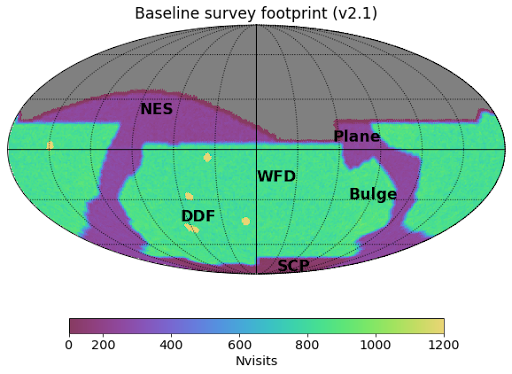
\includegraphics[width=0.5\textwidth]{figures/fp0.png}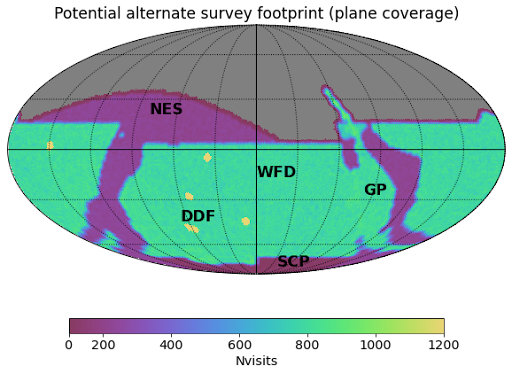
\includegraphics[width=0.5\textwidth]{figures/fp1.png}
    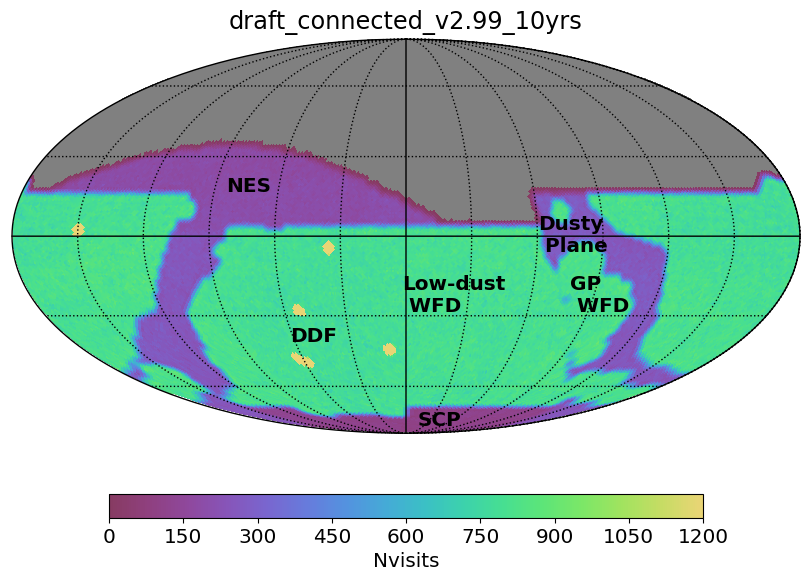
\includegraphics[width=0.5\textwidth]{figures/fp_299.png}
    \caption{Number of visits per field in three different \opsim\ simulations (colors saturated at 1,200 visits):  \texttt{baseline\_v2.1} (\emph{top left}); a simulation reproducing a TVS and SMWLV proposal for a prioritized Galactic Plane coverage, see \autoref{fn:TVSSMWLVFoot},
    (\emph{top right}), and the footprint plan for the baseline simulation presented in this report (\emph{bottom}).}
    \label{fig:fp}
\end{figure}

\begin{figure}
    \centering
    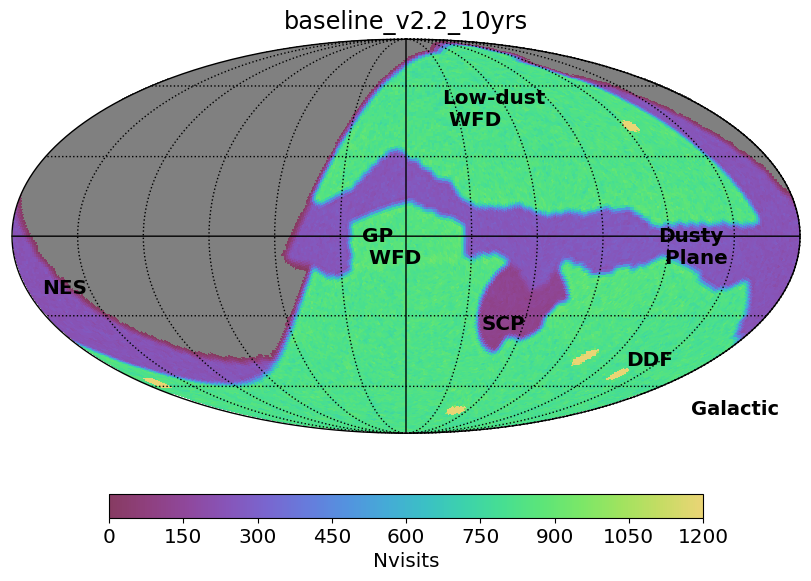
\includegraphics[width=0.5\textwidth]{figures/fp_200_gp.png}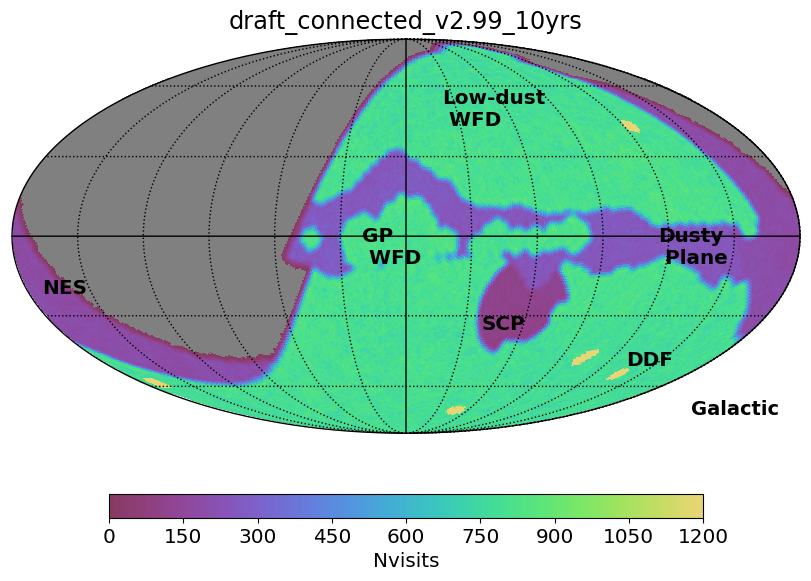
\includegraphics[width=0.5\textwidth]{figures/fp_299_gp.png}
    \caption{As \autoref{fig:fp} in a Galactic Plane projection for \texttt{baseline\_v2.2} (same footprint as \texttt{baseline\_v2.1}  \emph{left}) and for the current baseline (\emph{right}).}
    \label{fig:fp2}
\end{figure}

\subsubsection{SCOC recommendations: point by point answers}\label{rec:footprint}

\begin{enumerate}
\item 
The \texttt{baseline\_v2.X} WFD footprint appears to serve the scientific needs of the broad extragalactic community. The SCOC recommends that the \texttt{baseline\_v2.X} WFD low-dust footprint and overall time spent within it be preserved.

The current baseline implements an explicit WFD footprint request from DESC (which also benefits AGN, Galaxies, and extragalactic TVS science) to cover an extragalactic area of  $\sim18,0000~\degsq$ with $\ebv<0.2$~mag. To achieve this, \cite{2022ApJS..259...58L} recommended a footprint with $-70\degree<\mathrm{Dec}<+12.\degree5$
 over the portion of sky defined by the aforementioned extinction limit; an acceptable compromise, which avoids oversubscription of particular RA ranges and is adopted in the current baseline, is an upper limit of Dec~$<+15\degree$ for $\mathrm{RA}\sim7-18$~h and $\mathrm{Dec}<+3\degree$ for all other RA values.
 Synergies with other surveys (\emph{e.g.}, \emph{Euclid} and DESI) may motivate extending the survey declination limit even further into the northern sky, but there are currently no indicators that show strong benefits from this (metrics to measure the scientific advantages of overlap with these and other surveys while taking into account the expected image quality at high airmass should be developed to enable future reevaluations of the footprint northern limits). Nominal northern coverage of the Euclid region has been proposed as a microsurvey (\autoref{q:Micro}).

The SCOC recommends adding the Virgo Cluster to the WFD extragalactic region as part of the baseline survey (centered on RA$=186.75\degree$, Dec$=12.171$\degree, with a radius of $8.75\degree$).
Adding it represents a potentially important scientific payoff with negligible effects on the overall survey. Specifically, the addition of the Virgo Cluster in the WFD enables coverage of the highest stellar mass density in the nearby universe, with important benefits for local universe transient science and other key stellar populations such as globular clusters. Community support for this recommendation comes from the Galaxies SC (via their liaison).

\item As for the Galactic Bulge coverage and broader Galactic plane footprint, the SCOC is currently engaged in discussions with TVS and SMWLV representatives for further improvement (see above). \emph{ While no final recommendation is made for the Galactic plane footprint at this time, as described in \autoref{sec:shortrec} the distribution of observations within the Galactic footprint, including the filter balance and the different depth to which individual areas are covered, are compartmentalized decisions that can be optimized separately and do not significantly impact the rest of the survey.}

\item 
The SCOC recommends that the \texttt{baseline\_v3.0} simulation preserves the current \texttt{baseline\_2.X} total time allocation for the Galactic Plane. The amount of time spent observing the Plane as a whole in the current baseline represents the result of a compromise between competing scientific priorities and must be preserved in future strategies.  
%We did not find sufficient scientific support to justify taking a significant number of visits from the WFD, NES, or other minisurveys to allocate to the Plane. 
The distribution of visits within the Galactic Plane region and the Galactic Plane footprint are, however, a topic of active work and discussion (see point 2, as well as \autoref{q:Filters}, \autoref{q:Visits}, and \autoref{q:Rolling}).
%Therefore, additional time spent in the Plane should come primarily from other regions in the Plane/Bulge.


%However, it is possible that some additional time redistributed from the Bulge could be justified. We did not find sufficient scientific support to justify taking a significant number of visits from the WFD, NES or other minisurveys to allocate to the Plane: if the Plane is to have additional visits beyond the baseline, these should be reallocated from the Bulge.


\item The inclusion of the NES at the \texttt{baseline\_2.X} cadence level is supported by the SCOC. The SSSC metrics guide us in this recommendation.  A small reduction of NES coverage from the \texttt{baseline\_2.X} (from $\sim4.5$\% to $\sim3.5-4$\% of the survey time) is acceptable and it is implemented in \texttt{baseline\_v3.0}. Further changes at this level should be considered in a ``tweaking'' stage of the cadence in consultation with the SSSC. The current NES footprint extends from the northern boundary of the WFD and Galactic Plane up to $+ 10\degree$ ecliptic latitude; pushing this limit to lower ecliptic latitudes would lead to missing a substantial fraction of expected Solar System Objects (SSOs).

\item The SCOC recommends preserving the \texttt{baseline\_v2.0/2.1} time allocation for the SCP.
The main argument for the SCP is to allow for the opportunity to discover important Milky Way structures, such as dwarfs and streams, across the whole sky, making good use of Rubin as a survey instrument.  The current number of visits in the baseline is sufficient to have a significant scientific impact in this area, as can be seen from the Local Volume dwarfs metric and in the Local Volume notebook.\footnote{\url{https://github.com/lsst/rubin_sim_notebooks/blob/main/maf/science/Local_Volume_Dwarfs_Metric.ipynb}.} For example, compared to \citet{simon2019faintest}, LSST would probe new depths of dwarf discovery in the SCP, which is important for mapping the effect of the dark matter wake induced by the Large Magellanic Cloud \citep{garavito2021quantifying}. The exact filter distribution to be recommended for the SCP remains under investigation (see \autoref{q:Filters}).

\item 
To answer the question about the time to be spent on Galactic pencil-beam surveys, the SCOC needs more clarity on the definition of a pencil beam. Generally, we recommend balancing the benefits of segmentation of the Galactic Plane area into small subareas that serve niche science cases with the general benefits that LSST’s natural ability to cover large areas uniformly and deeply will afford. Outside of this balance being considered as part of the Galactic Plane/Bulge recommendation, pencil beams should perhaps be considered as micro- or nano-surveys (see \autoref{q:Micro}). Additionally, the use of alternative datasets (for example collected with DECam) that could complement LSST data and, if processed jointly, achieve specific science goals  should also be considered. \emph{At this stage the SCOC does not have a recommendation on the time to be spent on pencil-beam surveys of the Galactic Plane.}

\end{enumerate}


%\clearpage

\subsection{Filter Distribution}\label{q:Filters}

The Phase 1 SCOC report recommended implementing a single exposure for $u$ band visits (see \citetalias{PSTN-053} Q3), and maintaining overall visit times of 30 seconds for all other bands instead of variable visit (or exposure) times. Specific questions concerning filter balance, particularly considering a bluer skew of the survey (see \citetalias{PSTN-053} Q4), and more consideration of varying exposure time per visit were left to be addressed in Phase 2 report with the support of v2.X simulations. The specific questions to be addressed in the Phase 2 SCOC deliberations include:



\begin{enumerate}
\item Should the survey strategy skew towards bluer filter observations compared to the current baseline (bluer here is in reference to \texttt{baseline\_v1.7} and includes the consideration of additional coverage in either $u$ or $g$ bands)?
\item Should the same filter balance be applied to the entire LSST footprint (as opposed to, for example, implementing different filter balance in the extragalactic \emph{vs.} Galactic sky)?
\item What should the exposure time be for the $u$-band observations (including considerations of extending the $u$ band exposures to 50 seconds)? 
\item Should the survey use variable visit times or a set exposure time in each filter?
\item Should the survey use a different exposure than 2x15s (or possibly 1x30s) for non-$u$-band filters (for example, as implemented in the \texttt{shave\_filters\_v2.1} simulations)?
\end{enumerate}

\subsubsection{SCOC recommendations: executive summary }\label{rec:filterdist_es}

The SCOC has converged on most recommendations relating to filter distribution and has answered the questions left open in the Phase 1 report with the guidance of the reports and metrics provided by the community. Results on relevant metrics are included in a comparison notebook purposefully designed by the Survey Strategy team to guide filter-balance consideration \footnote{\url{https://github.com/lsst-pst/survey_strategy/blob/main/fbs_2.0/Filter\%20Balance.ipynb}}. {\bf The SCOC recommends to retain the filter balance and visit/exposure times as implemented in \texttt{baseline\_v2.X} on the WFD and tentatively in the Galactic Plane and Bulge, and SCP, although additional refinements on these and other minisurveys and special regions should continue to be considered. }

\subsubsection{SCOC recommendations: point by point answers }\label{rec:filterdist}

\begin{enumerate}

\item The SCOC recommends that the WFD filter balance implemented in \texttt{baseline\_v2.1}  be maintained in the low-dust WFD survey.\footnote{The depth by filter as implemented in simulation \texttt{baseline\_v2.0} is reported in \citep{PSTN-054} Table 3. The filter balance is essentially unchanged since \texttt{\baseline\_v1.7}.} Skewing the WFD survey strategy towards bluer filter observations would harm several science cases while providing benefits only to a few. 
SSSC and DESC science do not favor bluer filter observations (as presented in their reports).
The filter balance notebook\footnote{
\url{https://github.com/lsst-pst/survey_strategy/blob/main/fbs_2.0/Filter\%20Balance.ipynb}
} shows no strong support for a blue skew among the TVS metrics and indicates detrimental effects for cadence-dependent DESC metrics and SSSC metrics (examples of relevant SSSC metrics include Fraction LC inversion PHA H=16.0 and 19.0, Fraction LC inversion NEO H=16.0 and 19.0, Fraction LC inversion MBA H=16.0 and 18.0, Fraction LC inversion Trojans H=14.0 and 15.0). The v3.0 baseline implements this recommendation with the following ratios of median number of images in the WFD, compared to $r$ band: ($u$, $g$, $r$, $i$, $z$, $y$) $\sim$ (0.25, 0.35, 1.0, 1.0, 0.87, 0.90)


\item Conversely, although Galactic TVS science does not favor blue-enhanced $u$ and $g$ coverage, as it causes a detrimental decrease in performance for almost all regions,  different minisurveys as well as the Galactic Plane may benefit from changes to the default balance. \emph{The SCOC is not ready to produce a final recommendation for the filter balance for the Galactic Plane/Bulge or SCP region - we will continue working with the SMWLV and TVS SCs to find the best filter balance for Galactic science (see also \autoref{q:Footprint}).}

\item There is no evidence for significant performance improvements with either increased or variable $u$-band visit exposure length. We, therefore, recommend that the $u$-band 30 second exposure time implemented as a single 1x30s exposure visit so as to avoid becoming read-noise dominated \citep{PSTN-053},  be preserved.

As the basis for this conclusion, the SCOC considered several factors.  The reports from the SSSC disfavor the \texttt{long-$u$} simulation family. Simulations with the same number of $u$ visits as the \texttt{baseline\_v2.1} but a 50s exposure time showed enhanced results for X-ray binaries, the Galactic Bulge, and pencil beam fields in the $u$-band, but at the expense of observations in the other filters which are more important for most galactic transient science, which therefore does not overall favor longer or variable-length $u$ exposures. Increased $u$-band might lead to the enhanced discovery of new transient  extragalactic objects but may disfavor studies of kilonovae which are expected to be red in color (as reported in the TVS SC extragalactic science report).

The \texttt{long\_u2} simulations increase the exposure time for visits in $u$ without decreasing the overall number of $u$ visits, but at the expense of other bands, and this family of strategies is not strongly preferred by any science case reviewed by this committee.

\item There is no evidence for significant overall improvements by varying the exposure time (for example in response to observing conditions). In light of the additional expected complications in calibration and time-variability analysis if variable exposure times are introduced, the SCOC recommends against dynamically varying the exposure time. 

\item Conversely, the SCOC recommends revisiting the exact exposure length in each filter once the performance of the system-as-built is ascertained: it is possible that rebalancing the exposure time to compensate for performance and throughput in some filters as compared to others or shortening exposures in filters where the throughput exceeds expectations, enabling the collection of more images in that filter (or overall), could lead to enhanced LSST science. \emph{The SCOC cannot finalize this recommendation at this time due to missing information about the characteristics of the system-as-built}.

%\item The SCOC recommends against $u-$band observations longer than 30\,s, as implemented in the \texttt{baseline\_v2.1}.

%The reports from the SSSC disfavour the \texttt{long-$u$} simulation family. Simulations with the same number of $u$ visits as the \texttt{baseline\_v2.1} but a 50s exposure time showed enhanced results for X-ray binaries, the Galactic Bulge, and pencil beam fields in the $u$-band, but at the expense of observations in the other filters which are more important for most galactic transient science, so this is not preferred. Increased u-band might lead to enhanced discovery of new transient  extragalactic objects, but may disfavor studies of kilonovae which are red (as reported in the TVS SC analysis).

%The \texttt{long\_u2} simulations that increase the exposure time for exposures in $u$ without decreasing the overall number of $u$ exposures may be a fair compromise, but it is not strongly preferred by any science cases reviewed by this committee.

\end{enumerate}
\begin{figure*}
    \centering
    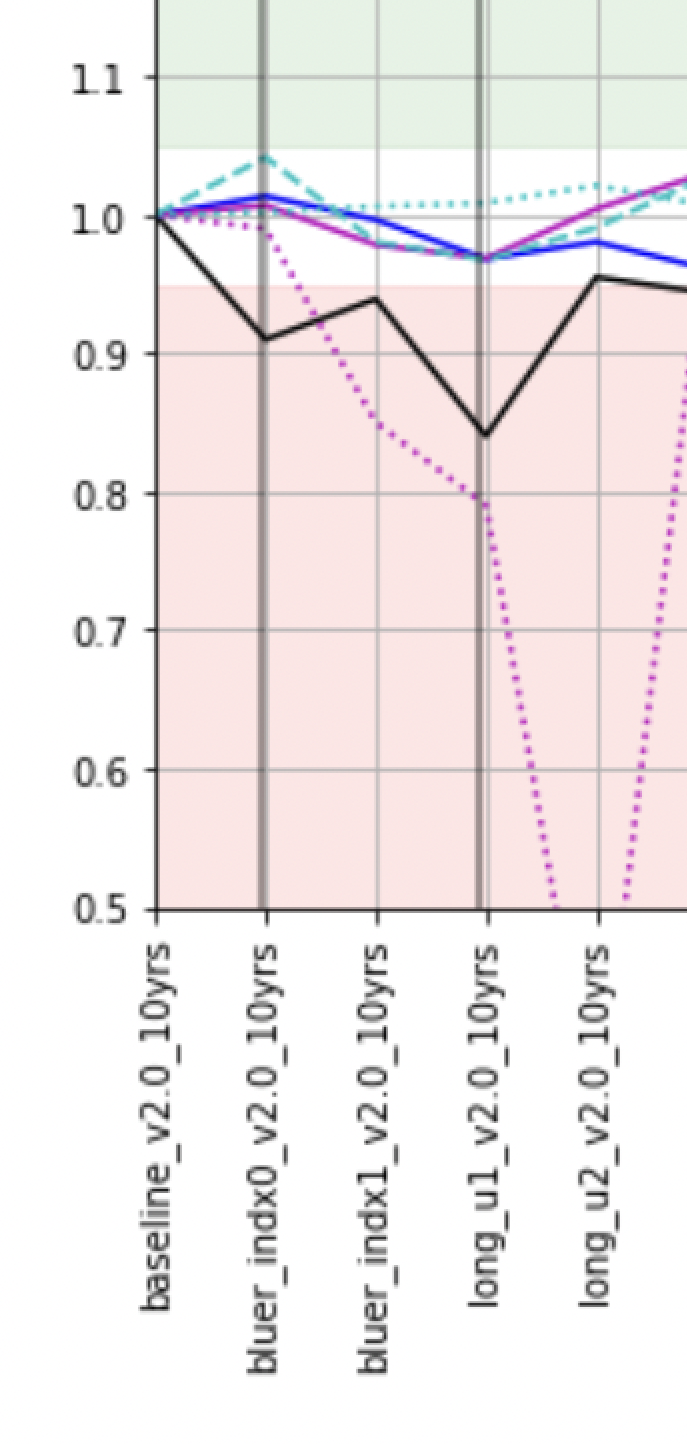
\includegraphics[width=1.7in]{figures/Filter_2.png}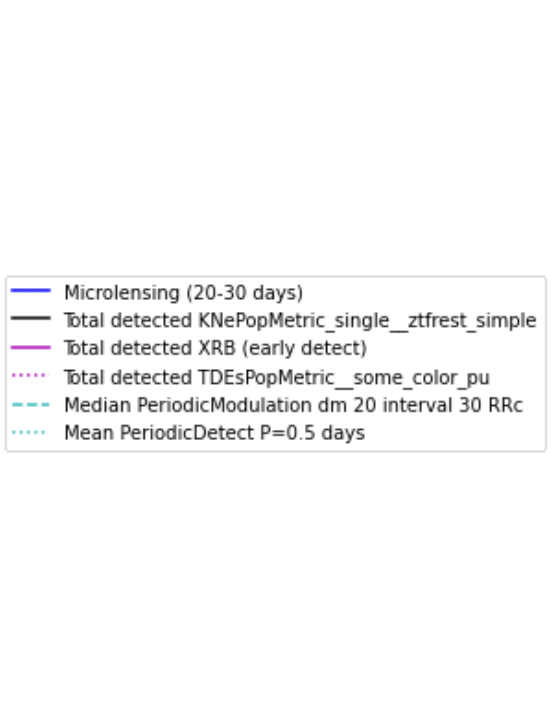
\includegraphics[width=2.5in]{figures/Filter1_Label.png}
    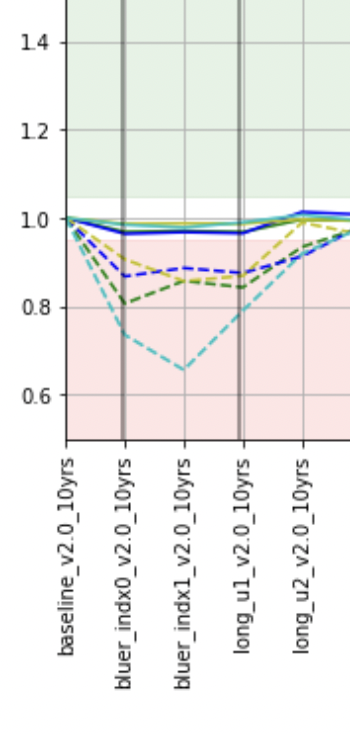
\includegraphics[width=1.7in]{figures/Filter_1.png}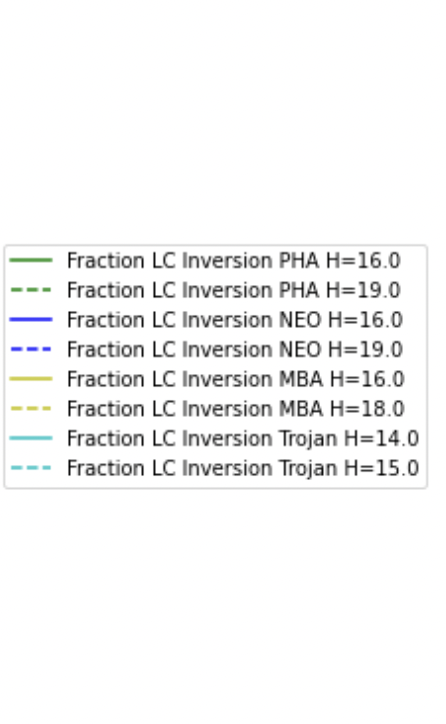
\includegraphics[width=2.3in]{figures/Filter2_Label.png}
    \caption{Impact of skewing the filter balance toward bluer filters for time-domain science metrics provided by the TVS SC (\emph{top}) and Solar System metrics provided by the SSSC (\emph{bottom}). The first point on the $x$ axis represents the benchmark performance of \texttt{baseline\_v2.0}, all simulations to the right of that skew toward bluer surveys by either increasing the fraction of observations in $u$ band or by increasing the length of the $u$ band exposures. In most cases the metrics are neutral or respond negatively to bluer implementations of LSST. The negative impact can be as significant as a 60\% drop in metric performance.}\label{fig:filterF1}
\end{figure*}
In addition, after the November 2022 SCOC workshop,\footnote{\url{https://project.lsst.org/meetings/scoc-sc-workshop3/home}} a request was made by the community (in particularly by members of the DESC) to make the $z$  filter more often available for observation: the Rubin Observatory filter wheel can house 5 of the 6 Rubin filters on any given night. The default plan as implemented in the v2.X simulations has been to swap $u$ and $z$ bands according to the moon phase. Availability of $z$ on the filter wheel on more nights produces smaller time gaps in the DDF observations (see \autoref{q:DDF}) in a wavelength range important for the characterization of high redshift SNe, with improved throughput for SN Ia cosmology. To support the DESC request simulations were made with the $u, z$, and $y$ filters alternating on the filter wheel. This minimally impacts filter balance but does impact the median time gaps for multiple filters as discussed in \autoref{q:Visits}. \emph{The SCOC recommends to continue the investigation of filter swap options while overall respecting the SCOC recommended filter balance}. 

%\clearpage


\subsection{Intra-night Cadence}\label{q:Visits}

The Phase 1 recommendations relevant to the intra-night cadence were primarily focused on how pairs of visits should be acquired and the exposure time for individual visits. The SCOC recommended that visits in each pair should be acquired in different filters, enabling the measurement of color information for transients and variables on short time scales. Investigations by the scheduler team found that pairs of visits separated by $\sim33$ minutes resulted in the best balance between minimizing filter changes and maintaining a high fraction of visits acquired in pairs (\citeds{PSTN-053} Q5) that enable SSO trajectory recovery. 

The questions left open after the Phase 1 recommendations on intra-night cadence were: 

\begin{enumerate}
\item Should there be a third visit in a night? Should it be all the time or only on some nights?
\item Should a third nightly visit be added everywhere in the sky (as opposed to for example only or preferentially in the extragalactic \emph{vs} Galactic regions or based on Ecliptic Latitude)?
\item If there is going to be a third visit on a night, what should the spacing between the second and third visits be?
\item If there is no third visit, what should the time separation between visits in a pair be (\emph{e.g.} 33 minutes or 2-7 hours)?
\end{enumerate}

\subsubsection{SCOC recommendations: executive summary}\label{rec:intranight_es}

The SCOC recommends increasing the number of field revisits on time scales of hours-to-one-day. Overall, these time scales are generally not well sampled by ``classic'' LSST cadences (see \citealt{2019PASP..131f8002B,2022ApJS..258...13B, 2022ApJS..258....2L}), yet they are important in the discovery and characterization of transients, as well as being largely unexplored by other surveys, especially at high redshift, and thus covering them increases the discovery potential of LSST.

Simulations that increase the number of visits on these time scales include the \texttt{presto\_color, long\_gaps}, and \texttt{suppress\_repeat} families. The \texttt{presto\_color} family includes a third visit to each field in the same night. The original implementation did not control the third visit time gap, and telescope efficiency considerations caused it to be taken in short time intervals. In \opsim\ v2.1, this parameter is controlled and visits are spread out by as little as 1.5 hours and as much as 4 hours. Note that the original paper proposing a presto-color-like cadence \citep{2019PASP..131f8002B}\footnote{Originally submitted as a white paper in response to the 2018 Cadence White Papers call.} did \emph{not} recommend revisits on time scales $<4$ hours as those time scales are too short to meaningfully constrain flux evolution even for (known) rapidly evolving transients, thus the scientific benefit of this family of simulations is not clear. Nonetheless, this family of simulations with an increasing time gap for the third visit reveals important trends in response to the addition of a third visit which we discuss in the next paragraph. The \texttt{long\_gaps} family of simulations implements repeat visits on longer time scales, implemented both in visit triplets and in visit pairs (\emph{i.e.} separating the pair by several hours).
An additional relevant family of simulations is the \texttt{suppress\_repeat} which actively suppresses the third visit in a night. By preventing the scheduler from taking these third visits it forces it instead to take other less-preferred observations, including fields that were observed on the immediately prior night. Thus this family further undersamples the timescale between 33 minutes and 12 hours, but increases the sampling at $\sim$24 hours. Finally, it should be noted that the implementation of a rolling cadence also helps reduce the minimum revisit time gap and increases the number of images that fall into the hours-to-one-day time scales.


Scientific metrics that are sensitive to these cadences include the kilonova metrics, as well as metrics designed to detect rare and unusual phenomena (Presto- and Presto-Color metrics, not to be confused with the \texttt{presto-color} family of simulations). Generally, we found all these metrics benefit from the inclusion of a third visit and to steadily improve as the time gap is increased up to several hours or into the following night. However, including a third visit to the same field within a night has an impact on survey efficiency because it adds a constraint on the selection of target fields that may take precedence over image quality and slew time considerations. Thus most metrics sensitive to image quality or to the number of images collected are negatively affected if third visits in the same night are required extensively. For example, many SSSC metrics including detection fractions and light curve inversion metrics for the different Solar System populations
 perform poorly on the \texttt{presto\_color} family of simulations, especially when the time gaps are short and the constraints on field selection are tighter. In addition to these specific scientific metrics, the TimeGaps metric (\autoref{fig:tgaps}) provides a science-case-agnostic gauge of the number of revisits that fall in this range of revisit timescales.


{\bf With these considerations, the SCOC converged on recommending that visit pairs be maintained within a $\sim33$ minutes time scale, with different filters, as implemented in the \texttt{baseline\_v2.0} and most v2.X simulation (see \autoref{sec:v3} for details on the band pairing, which may be subject to further study).
This time spacing is critical for Solar System science, and the different filters provide a color measurement useful for transient characterization. Further, the SCOC recommends the LSST cadence be designed to ensure coverage of time scales in the hours-to-one-day range by carefully tuning survey parameters in combination. Performing three visits per night by default is not recommended, but a combination of preferentially pushing a third visit to the following night (which can be achieved by implementing a rolling cadence, see \autoref{q:Rolling}, in conjunction with the suppression of a third nightly visit as done in the \texttt{suppress\_repeat} family of simulations) and requesting a third visit within a night once every several nights ($\sim1$ week) would achieve this goal.
It is important these third visits be taken in one of the bands that were already observed in the visit pair.}

It is hard to better quantify at this time the precise amount of time or number of visits that should be spent on the hours-to-one-day revisit time scales. The discovery potential in this region is obvious and driven by the fact that these time scales are currently poorly explored, particularly at the high redshifts that LSST will reach. The investment in these time scales should be reevaluated regularly throughout the survey. 

We further note that, while a third visit during the same night can plausibly be a single visit (i.e. not a pair separated by 33 minutes), next-night observations may need to be paired to preserve the ability to use the visits for linking Solar System objects (\emph{i.e.} third and fourth visits).

\subsubsection{SCOC recommendations: point by point answers}\label{rec:intranight}

\begin{enumerate}

\item The third visit within the same night should be implemented for only a small fraction of observing time. The SCOC tentatively suggests implementing third visits for one night out of every 7 nights, but this could also be distributed in other ways at a similar total time fraction (see also \autoref{q:Rolling}).

\item Since the scientific motivation for the implementation of the third visit is broad and includes the discovery of unknown, unexpected phenomena, there is no strong motivation to limit the third visit to some areas of the sky. But we note that the SCOC has suggested specific exploration of survey parameters, such as footprint and filter selection, that would enhance Galactic science (see \autoref{q:Footprint} and \autoref{q:Filters} ). \emph{Similarly, if Galactic science can demonstrably be enhanced by a different intra-night cadence this recommendation may change outside of the low-dust WFD footprint}.


\item Because a goal of having three visits in one night is to ensure coverage of a phenomenon over a range of timescales, we recommend that third nightly visits be broadly distributed in the 2-7 hour range rather than on a rigid cadence.
We also encourage some small fraction of revisits on the immediately following night, to further improve measurements on timescales faster than three days.
This is consistent with the recommendations from several cadence notes (\citealt{2022ApJS..258...13B},\footnote{\url{https://docushare.lsst.org/docushare/dsweb/Get/Document-37644/Delta_T_2021.pdf}.} \citealt{2022ApJS..258....2L},\footnote{\url{https://docushare.lsst.org/docushare/dsweb/Get/Document-37653/Anomalies.pdf}.}, and Richards et al. 2019\footnote{\url{https://docushare.lsstcorp.org/docushare/dsweb/Get/Document-30572/richards_agn_rolling_wfd.pdf}.} as well as \citealt{2019PASP..131f8002B}.


\item 
The science goal of many of the third-visit proposals is to obtain both a color and a rate of change, and increasing the time separation of visit pairs is insufficient to meet these requests.
The revisit time within pairs was already addressed in the SCOC Phase 1 recommendations. Thus the SCOC recommends that the visit pairs be preserved as designed in the v2.X simulations with a goal of $\sim33$ minutes separation.


\end{enumerate}
\begin{figure}
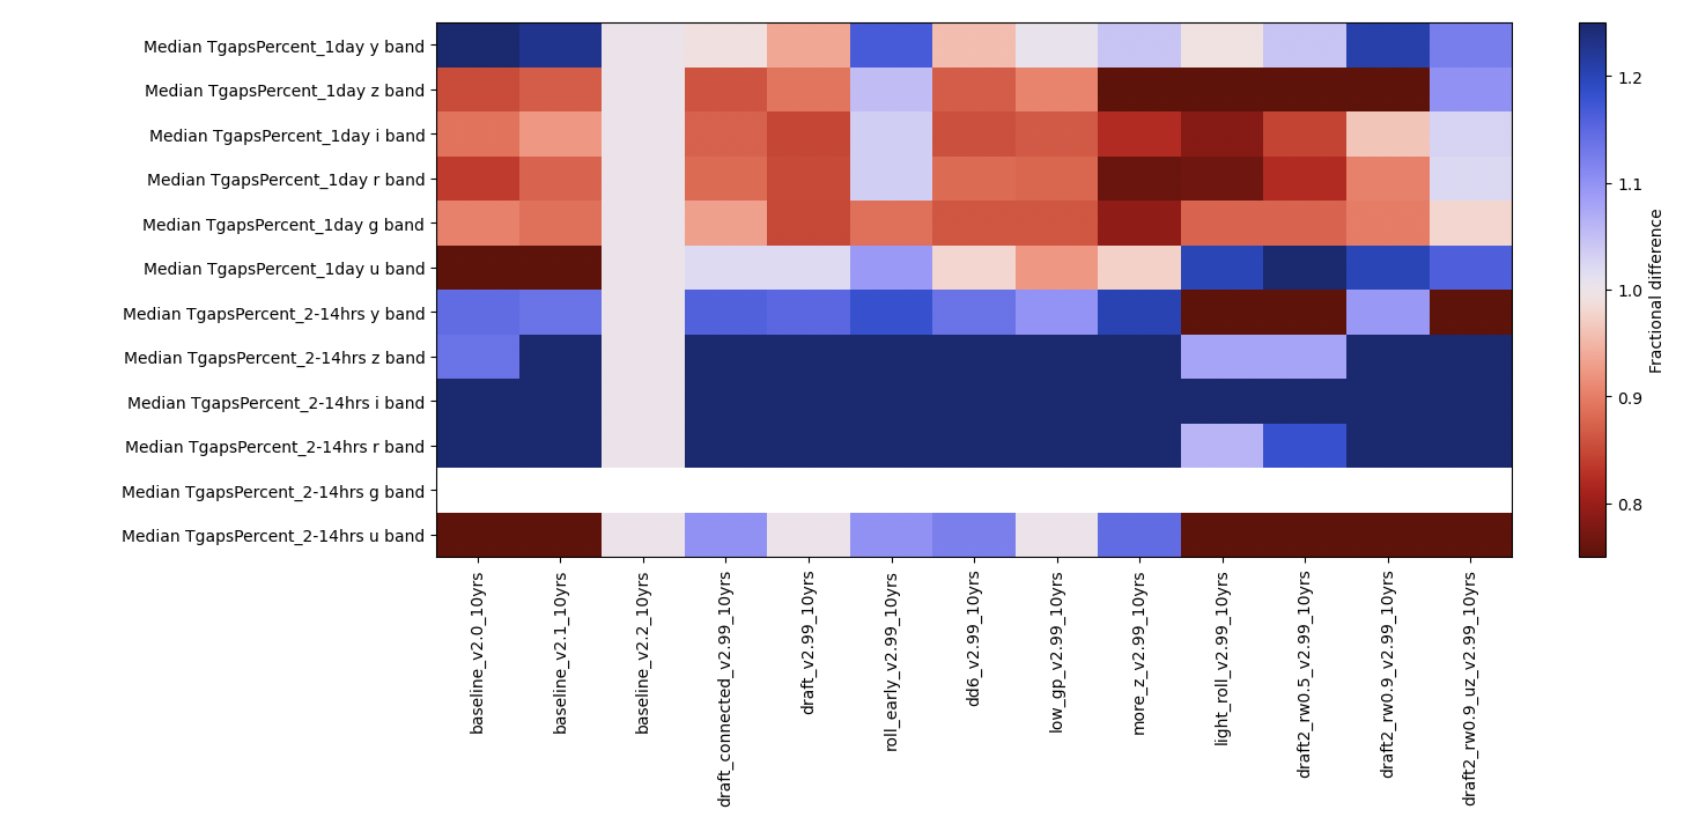
\includegraphics[width=0.95\textwidth, right]{figures/tgaps.png}
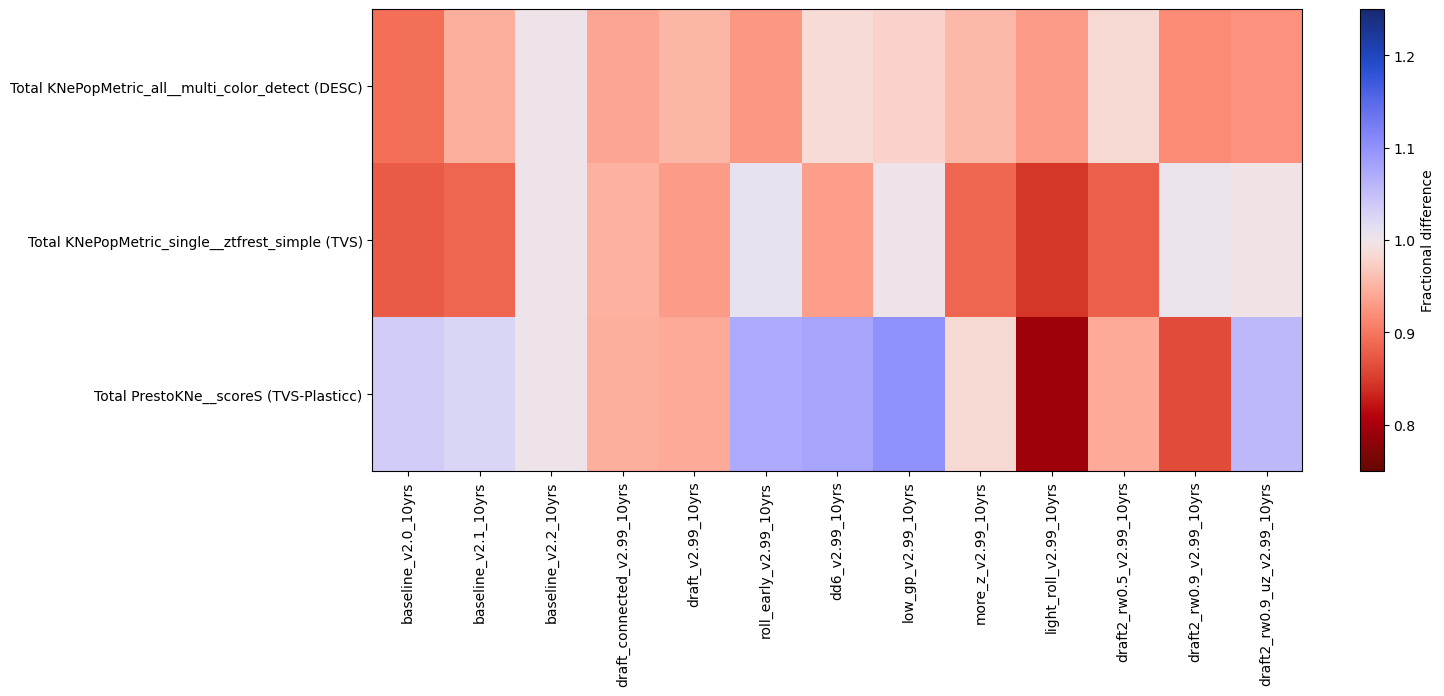
\includegraphics[width=0.94\textwidth, right]{figures/kne.png}
\caption{The response of metrics sensitive to intra-night cadence to the v2.X baselines and the v2.99 simulations. The performance is benchmarked in both plots with respect to \texttt{baseline\_v2.2}. Top: metrics showing the fraction of visits falling in the 2-14 hours and one day time ranges for different filters; bottom: three kilonovae metrics. Note: the simulation appearing here as \texttt{draft\_rw0.9\_uz\_v2.99\_10yrs} was subsequently adopted as \texttt{baseline\_v3.0}.}
\label{fig:tgaps}
\end{figure}

A final point should be made about the relationship between the time-gap distribution and the filter exchanges. As noted in \autoref{q:Filters}, the Rubin filter wheel can host 5 of the 6 filters on any given night. Which filters should be swapped and when is under discussion and some science cases (SN Ia cosmology in particular) benefit from increased access to some bands (\emph{e.g.} $z$) to reduce time gaps between sets of observations (particularly in the DDFs, \autoref{q:DDF}). However, the choice of filters on the wheel impacts more than the specific filters that are involved in the swap, due to the prescribed pairing of filters for the observation pairs, themselves driven by efficiency considerations including pairing filters suited to observe under similar conditions and enhancing the discoverability of SSOs (see \autoref{sec:v3}). \emph{As indicated in \autoref{q:Filters}, the filter swapping strategies deserve more attention, and we recommend that the impact of these choices on time gaps in all filters be monitored when alternative filter change strategies are tested in simulations}.

%\clearpage

\subsection{Rolling Cadence} \label{q:Rolling}

The Phase 1 SCOC report included a recommendation to adopt a half-sky rolling cadence and to continue to investigate rolling options. With the expansion of the footprint recommended in Phase 1 (see \autoref{q:Footprint}), the number of visits per pointing in the WFD dropped slightly, with an associated impact on metrics dependent on cadence in the few days range. The inclusion of rolling in the cadence, which concentrates visits into some region of sky during some seasons at the expense of visits' cadence during other seasons, was intended to counter this drop in cadence near the 3-5 day range (see \citetalias{PSTN-053} Q6).


The questions left open after the Phase 1 recommendations on rolling cadences were: 

\begin{enumerate}
\item Should a rolling cadence be adopted in the WFD?
\item Should a rolling cadence be adopted in the special regions of the WFD (NES, GP, SCP) and minisurveys?
\item Which scheme for rolling should be adopted? (number of rolling regions, other spatial region splits)
\item How aggressive should the strength of the rolling be in the WFD or non-WFD footprint?
\item When should rolling start (end of year 1 or after 1.5 years)?
\end{enumerate}

\subsubsection{SCOC recommendations: executive summary}\label{sec:rolling}

 The SCOC reviewed metrics from the community, especially as presented in notebooks that compared the performance across v2.X simulations and earlier baselines.\footnote{See: \url{https://github.com/lsst-pst/survey_strategy/blob/main/fbs_2.0/Rolling\%20Cadence.ipynb} and \url{https://github.com/lsst-pst/survey_strategy/blob/main/fbs_2.0/Rolling\%20Cadence\%20v2.2.ipynb}.} Following the Phase 1 SCOC recommendations, rolling is implemented as a default in v2.X simulations with a split into two half-sky regions defined by declination limits and with a $\sim0.9$ rolling weight\footnote{The weight is the relative fractions of images that the scheduler is requested to schedule on the active \emph{vs} inactive regions of sky. However, it should be noted that additional constraints on the number of images (\emph{e.g.}, collection of a sufficient number of images over time to enable the creation of templates) are likely to cause the number of images actually collected to differ from this request.} \citepalias{PSTN-051}. {\bf While some details remain to be optimized jointly with other SCOC choices, the SCOC recommendation is for a half-sky 0.9-weight rolling cadence on the WFD and, tentatively, on the Galactic Plane and Bulge as well, as a practical compromise to support both static-sky science and time-varying science.    
This recommendation is made under the assumption that sufficient uniformity in depth to support static-sky cosmology (and more in general, static-sky science) in annual data releases can be achieved in data-processing.  Should this not be the case, the SCOC will re-evaluate this recommendation.}


 \begin{figure}
    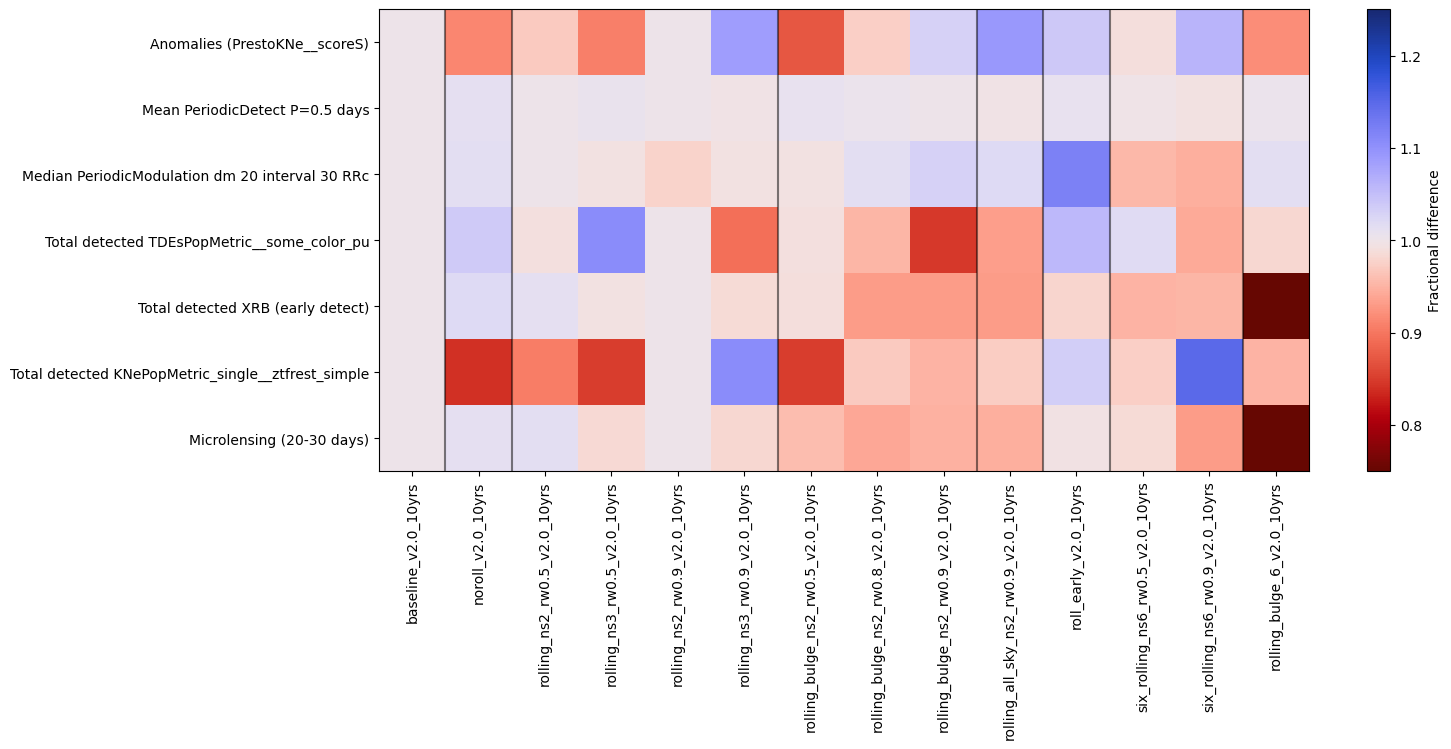
\includegraphics[width=\textwidth, right]{figures/roll_tvs.png}
     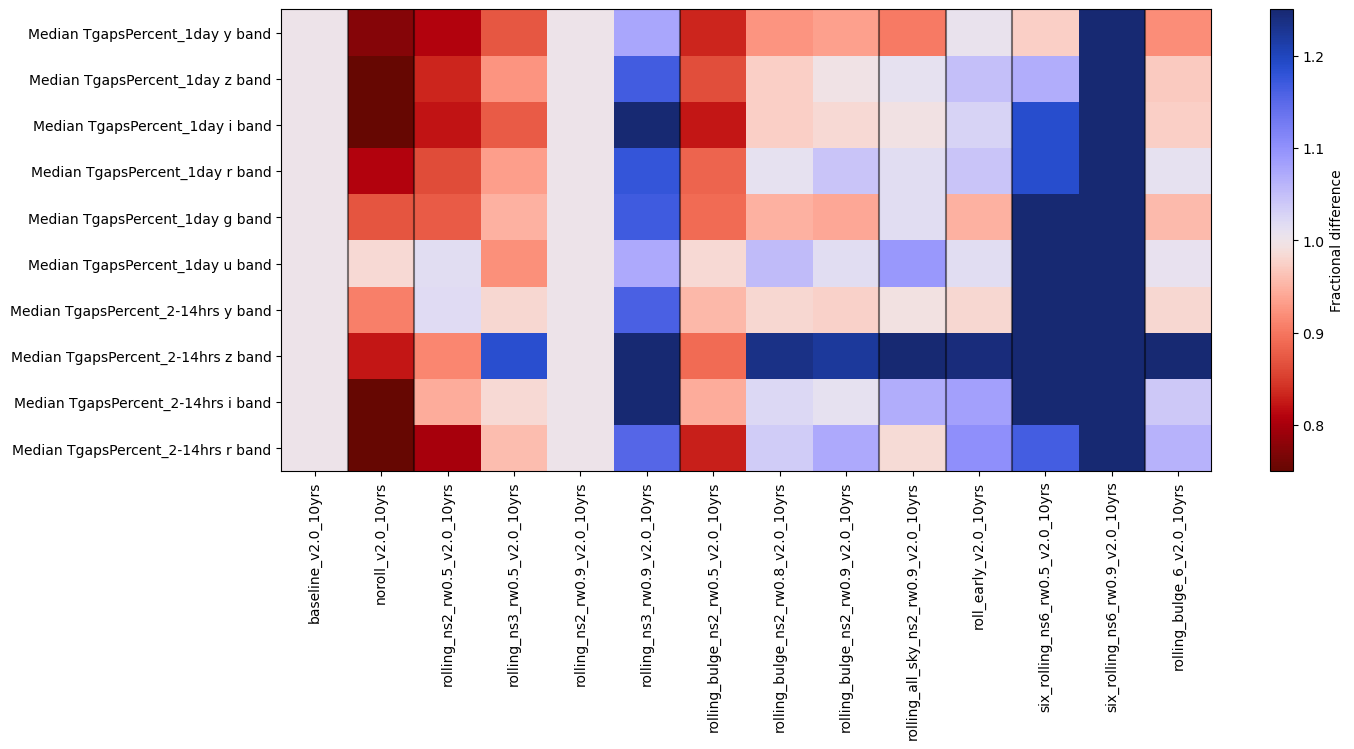
\includegraphics[width=0.93\textwidth, right]{figures/roll_tgaps.png}\caption{Some of the metrics considered in deliberating about a rolling strategy for LSST and their performance for selected 2.0 simulations (the reference simulation for both plots being \texttt{baseline\_v2.0}, which implements half-sky rolling at 0.9 weight). Top: time-domain metrics. While time-domain metrics that monitor long transients (e.g. TDE) prefer weak or no rolling, rapid transients strongly prefer rolling (kilonovae and anomalies metrics). This is because of the additional coverage on time scales $<2$ days, as seen in the bottom panel which shows the percentage of observations following in specific time scales with specific filters. However, very aggressive rolling, for example in 6 sky areas (\texttt{\_ns6\_}), is strongly disfavored by many time-domain metrics because of the reduced survey efficiency due to additional constraints on pointing.}
     \label{fig:knroll}
 \end{figure}

 \subsubsection{SCOC recommendations: point by point answers}\label{sec:rolling_points}
 


\begin{enumerate}
    \item 
The SCOC supports a rolling cadence\footnote{A cadence where a portion of the sky is emphasized in one rolling cycle, to then be de-emphasized in the following rolling cycles.} and recommends that rolling be adopted across the WFD. Our recommendation is based on the review of the metrics and reports from all SCs. Transient metrics for the extragalactic sky strongly support rolling. A non-rolling cadence would negatively affect all extragalactic transient metrics presented by TVS, typically by 20\%.
 The DESC supports a rolling cadence as it is shown to improve the sampling of SN Ia light curves for cosmological characterization (see Sec 9.5 and Fig 9.22 of \citealt{cosep} and \citealt{https://doi.org/10.48550/arxiv.2210.15690}). The SSSC and AGN SC metrics perform well or neutrally with some rolling, although the strength of rolling has to be decided carefully, and we return to this point in our response to points 3 and 4. 
 
 \item \emph{The SCOC does not have a final recommendation for rolling on the Galactic Plane/Bulge at this time}. The decision about rolling in this area is compartmentalized and should not impact the WFD performance, though this assumption has to be verified via simulations. Thus the SCOC can continue to optimize the rolling choices on the Galactic Plane, together with the details on the filter balance and footprint over the Galactic Plane (\autoref{q:Footprint} and \autoref{q:Filters}). The current implementation of rolling on the Galactic Plane with the same scheme adopted in the WFD seems, however, to be a good compromise to support short- and long-variability phenomena (see below). No simulations with rolling on the NES and SCP or minisurveys have been created to date. The NES and SCP have fewer visits and may therefore not benefit from rolling, and it may not even be possible to implement rolling while also producing adequate annual templates. 

 \item Questions 3 and 4 will be discussed jointly: 
 
 \item The decision about the strength of rolling concerns both the number of areas over which rolling occurs and the weight of the rolling (the fraction of the time spent on the on \emph{vs} off sky regions).  The SCOC has reviewed combinations of rolling implemented on sky splits into 6 rolling regions, 3 rolling regions, and 2 rolling regions (or half-sky) and at 0.5, 0.8, and 0.9 rolling weight in v2.X simulations. When analyzing the strength of a rolling cadence, in the segmentation of the sky or in the rolling weight, SCOC considerations, guided by the community metrics, include the impact on transient phenomena characterization at all time scales (\autoref{fig:knroll}), but also the impact on the uniformity of the data releases in terms of coverage and depth (\autoref{fig:rolluniformity}). In particular: the DESC science requires a certain degree of uniformity in intermediate data releases for static sky cosmology and the DESC urged, via its reports\footnote{\label{fn:descreport}\url{https://lsst.org/sites/default/files/documents/DESC-SCOC_November2022.pdf}} and its liaisons, that Rubin intermediate data products (galaxy catalogs, etc.) be made from as uniform-depth extragalactic WFD data as possible. This is likely to be a concern for other static-sky science as well, such as the science relevant to the Galaxies SC and Strong Lensing SC. \emph{A measurable definition of the required uniformity and evaluations of the data processing options to achieve it should be undertaken in 2023}. AGN metrics for detecting Blazar time lags are insensitive to rolling cadence but can underperform if objects are poorly characterized due to the long gaps in coverage, which would happen in the off-sky regions for aggressive rolling patterns. The AGN Structure Function metric also sees an increase in errors with 6 sky areas identified for rolling (``6-band'' rolling). Finally, with such high sky segmentation, slow-evolving transients would be poorly characterized (although most transient metrics focus on fast transients and early transient characterization and may not reflect this concern). In addition, adding constraints on the pointing reduces the efficiency of the survey by reducing the ability to select a position on the sky that minimizes slew and that maximizes image quality. Thus most metrics, including time-domain metrics, suffer when aggressive rolling schemes with high sky segmentation are implemented (\emph{e.g.} in sky sixths, or ``6-band'' rolling) because of the overall reduced number of images and survey depth. Therefore, the SCOC overall disfavors an aggressive ``6-band'' rolling cadence.
 \begin{figure}
    \centering
    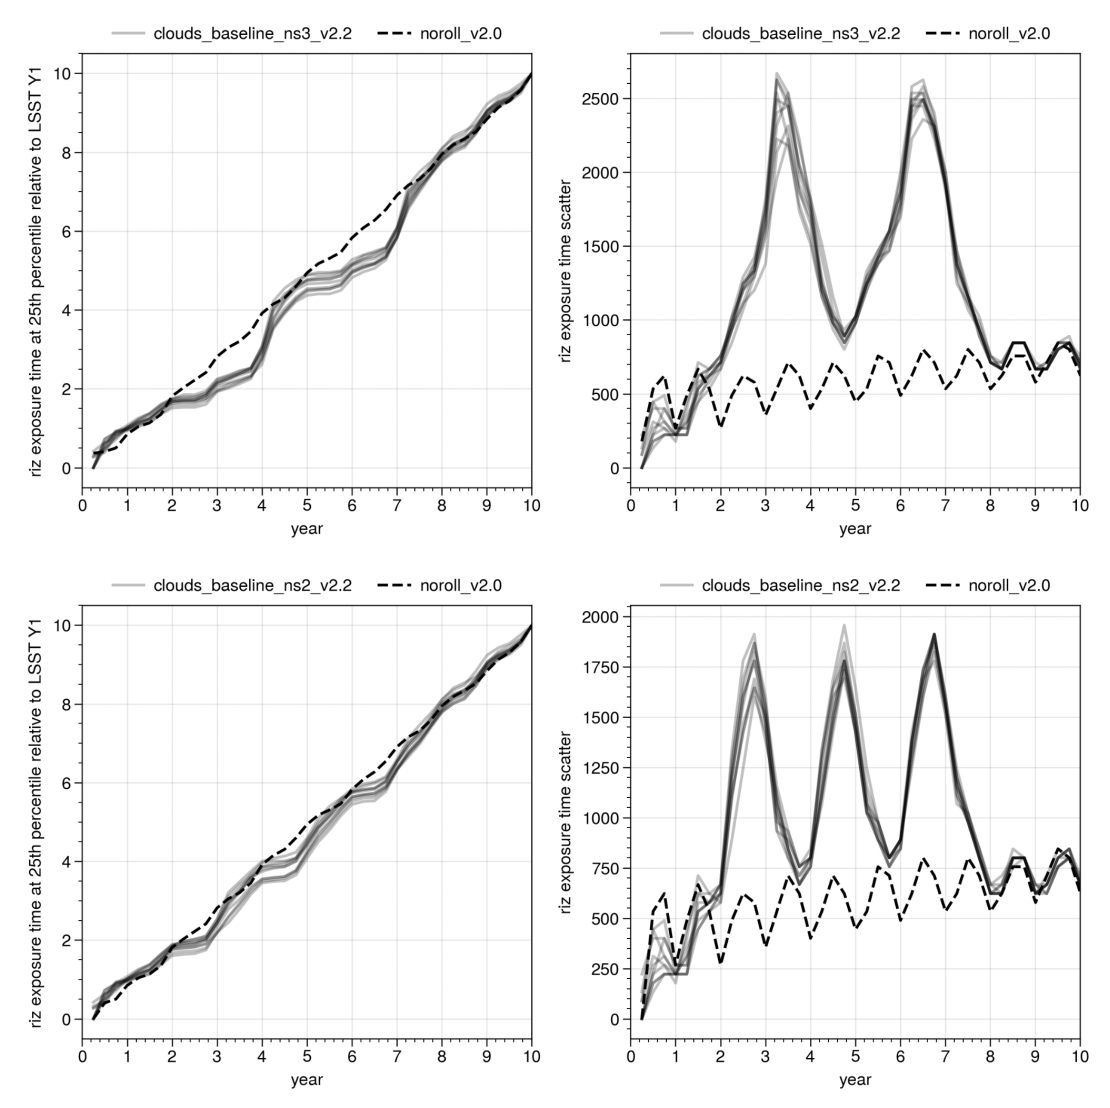
\includegraphics[width=0.6\textwidth]{figures/uniformity_DESC.png}
     
     \caption{Uniformity of annual data releases (produced by M. Becker, DESC, see \autoref{fn:descreport})
     : \emph{Left}: cumulative exposure time per sky region relative to year 1; \emph{right}: scatter in the exposure time.
     Rolling cadences in sky thirds (\texttt{cloud\_baseline\_ns3\_v2.2}, \emph{top}) and half-sky rolling (\texttt{cloud\_baseline\_ns2\_v2.2}, \emph{bottom}) with a 0.9 weight, where rolling begins after year 1, shown against a non-rolling simulations (dashed line). The rolling strategies are shown for multiple simulations with varying cloud patterns. Rolling over half the sky has a significant impact on the uniformity needed for static science in years ~3, 5, and 7, but recovers in years 4, 6, and 8. A rolling scenario with sky segmentated into thirds (sometimes referred to as ``3-band'' rolling) causes significant degradation in uniformity over years 3, 4, 6, and 7, and the recovery of uniformity by year 5 is not as complete as in the half-sky case. }
     \label{fig:rolluniformity}
 \end{figure}

  While splitting the sky into thirds (earlier referred to as ``3-band'' rolling scheme) and rolling at a 0.9 weight would produce a good sampling of transients, including fast transients such as kilonovae by covering short time scales (see Kilonova metrics, \autoref{fig:knroll}, top), it would negatively impact metrics measuring data release uniformity (see the November 2022 DESC report\footnote{\url{https://lsst.org/sites/default/files/documents/DESC-SCOC_November2022.pdf}} and \autoref{fig:rolluniformity}) and Strong Lensing metrics. Conversely, a half-sky 0.9 weight rolling strategy \emph{alone} would leave time scales between 2-14 hours and one day undersampled and unexplored, with decreased performance on fast transients and potential loss of discovery (\autoref{fig:knroll}, bottom). However, as discussed in \autoref{q:Visits}, choices that control the intra- and inter-night cadence could solve the hour-to-one-day time scale issues and be jointly applied with rolling to achieve optimal results.  %To confirm that this is indeed optimal, we require a few simulations to be produced explicitly tuning these parameters.  
  The current SCOC recommendation is for half-sky rolling and 0.9 rolling weight. The optimization of rolling parameters is intertwined with the choice of intra-night cadence and repeat observations and triplets every few to several days and observations on the following day performed often in combination with this rolling scheme are likely to achieve the desired results. Note that in a half-sky rolling scheme the sky is actually split into 4 regions defined by declination, of which two are active at a given time (see \autoref{sec:v3}). 
  
  The new baseline represents a significant relative improvement over previous implementations of a rolling cadence but further refinement could help boost the low absolute numbers of visits in underexplored and poorly explored times scales. Therefore, this recommendation should not be interpreted as final; joint optimization of the observation repeat pattern and rolling should be continued by the SCOC. 

  \item Rolling should start after the first part of the sky which has had a complete season of observations
in “uniform” cadence starts its second season. That is roughly 1.5 years after the start of the survey. Early rolling (\emph{e.g.}, starting at or near the end of year 1) would lead to severe non-uniformity that would compromise DESC early science.\footnote{See \autoref{fn:descreport}.}

\end{enumerate}

%\clearpage

\subsection{DDF Strategy}\label{q:DDF}

Details of the survey strategy for the DDFs were not directly tackled during Phase 1. The questions defined during Phase 1 related to DDFs were:

\begin{enumerate}
\item How much survey time should be spent on the DDFs?
\item Should all DDFs be observed for the entire 10 years?
\item Should some DDFs get more observations in certain years and none/less in others? If so, which ones and in which years do those fields get observed?
\item Should the Euclid South DDF be finalized as the 5th field (what else do we need to know about observing and co-observing needs)? 
\item Should the Euclid South DDF be observed differently than other DDFs?
\end{enumerate}
 
 \subsubsection{SCOC recommendations: executive summary}\label{sec:ddfes}
 
The SCOC based its recommendation on metrics and feedback from the SCs,  feedback on community.lsst.org, feedback through the SCOC liaisons, and feedback in the November 2022 SCOC workshop. The AGN SC, Galaxies SC, SLSC, and the DESC have provided recommendations. 


 
{\bf The SCOC recommends that no less than 5\% of the survey be dedicated to DDFs, with the potential to increase this fraction to as high as 7\%. The SCOC recommends the selection of the Euclid Deep Field South as the 5th DDF, with a footprint that can be covered with two LSST pointings, each to be observed at 1/2 of the depth of the other DDFs. That all DDFs be observed for 10 years and the COSMOS field is observed to full 10-year depth within the first 3 years of LSST and continues to be observed thereafter at the same rate as the other DDFs.} The typical DDF 10-year coadded depth in the current implementation of these recommendations (see \autoref{sec:v3}) reaches 1.3 magnitudes deeper than the coadded WFD depth in the same band. At this stage, the inter- and intra-night cadence for DDF observations remains to be defined and few metrics are available to evaluate its performance. %With that in mind, the current recommendations on the specific intra-night cadence to be implemented are as follows. 
To support transient science, including cosmology through SN Ia, the intra-night cadence of the DDF observations need to support effective characterization of SNe. For SN Ia cosmology specifically, observing DDFs for the entire ten years of LSST is only optimal  if this can be done with a cadence that avoids large time gaps between DDF observing nights. \emph{The SCOC will continue working in 2023 with the community to identify the specific intra-night cadence that maximizes the science throughput of the DDF survey, while not impacting the science performed through the rest of the LSST, including and in particular within the WFD.}
 
 \subsubsection{SCOC recommendations: point by point answers}\label{sec:ddf_points}
 
\begin{enumerate} 
\item The SCOC recommends no less than 5\% of the survey time be spent on DDFs, with consideration of going up to 7\% balanced against other demands such as the total number of WFD visits. Our recommendation is based primarily on the review of the metrics and reports from the SCs. The DESC, Galaxies and AGN SCs all recommend strong investment in the DDFs. SN Ia cosmology at high redshift (giving the best constraints on the dark energy equation of state variation $w_a$) requires deep observations. AGN reverberation mapping benefits from consistent coverage in the DDFs at least at the 5\% level. The Galaxies SC prefers deeper DDFs (>5\%) to probe fainter galaxy populations, both lower mass galaxies nearby as well as galaxies at higher redshifts. We believe the scientific return of a $>5\%$ investment in DDFs is well justified, and simulations demonstrate that devoting $\sim7\%$ of the survey time to DDFs can be achieved while ensuring good performance on the WFD and fulfillment of the survey requirements \citeds{LPM-17}.

\item The SCOC recommends that all DDFs should be observed for the entire ten years. AGN variability amplitude correlates (roughly linearly) with time, leading to the identification of many more faint AGN (often blended with their host galaxies) over longer baselines. Likewise, proper motion metrics benefit from longer overall baselines. COSMOS is the closest DDF to the ecliptic, so SSSC prefers $>2$ years of observations in the COSMOS DDF to reduce orbit uncertainties. 
This justifies the requirement to maintain long overall baselines.


\item There are specific reasons for starting the DDF observations early and collecting a substantial amount of DDF data early in the survey: the DDF DESC photo-z calibration will be enhanced by the earlier information that can be obtained in the DDFs; the Galaxies SC also argue for at least one DDF to be completed early for low-surface-brightness science and calibration purposes: as Rubin will reach unprecedented photometric depths, the methodology for low-surface-brightness science remains to be developed and its development may lead to insight in the optimization of subsequent DDF observations. 
The SCOC recommends that the COSMOS DDF be prioritized with additional survey time front-loaded to reach 10-year DDF depth on COSMOS within the first three years of LSST. The selection of the COSMOS field among the other DDFs to implement this deeper and front-loaded observing plan is guided by recommendations of both Galaxies SC and DESC and is driven by the broad availability of ancillary data and its location.



\item As announced on community.lsst.org,\footnote{\url{https://community.lsst.org/t/scoc-endorsement-of-euclid-deep-field-south-observations/6406}} the SCOC recommends that the Euclid Deep Field South (EDFS) be selected as the 5th field. The EDFS covers an area roughly twice as large as the 9.6\degsq\ pointing of Rubin, which is the extent of each of the other DDFs. The SCOC recommends that the EDFS be observed at half-depth over its full area.
This recommendation is based on the feedback from the Galaxies SC, which recommends as much overlap with Euclid as possible, and the Euclid-LSST Derived Data Products Working Group \citep{https://doi.org/10.5281/zenodo.7195671} that strongly prefer this option. 

\item
 \emph{Work, in coordination not only with the scientific community but also with the leadership of Rubin and Euclid remains to be done to identify cadence requirements and co-observing strategies, which may lead to modifications of the timeline for the EDFS data collection, and paths to ensure support for the generation of data products that will enhance science through the coordinated observing of the EDFS.}


\end{enumerate}

\begin{figure}
    \centering
    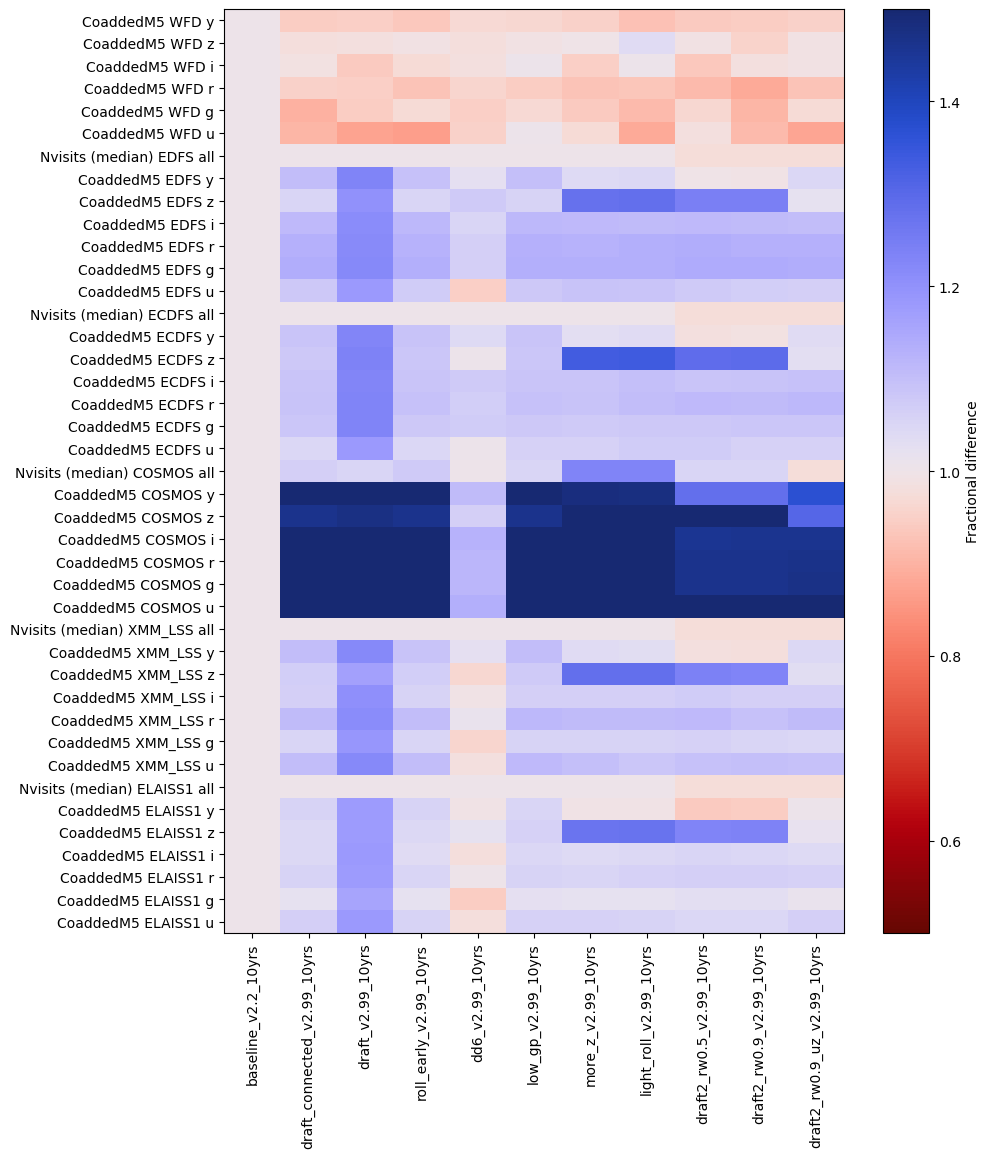
\includegraphics[width=0.6\textwidth]{figures/ddf.png}
    \caption{Coadded 10-year depth (magnitude) of the WFD and each the five DDFs that LSST will observe in each band for \texttt{baseline\_v2.2} (used as reference) and a set of v2.99 simulations. Note the increased depth for the COSMOS field, as per SCOC Phase 2 recommendation, and the inclusion of the EDFS in the final set of LSST DDFs. The filter balance in the DDFs can be tweaked, independently of the filter balance in the WFD. Note: the simulation appearing here as \texttt{draft\_rw0.9\_uz\_v2.99\_10yrs} was subsequently adopted as \texttt{baseline\_v3.0}.}
    \label{fig:my_label}
\end{figure}

%\clearpage

\subsection{Microsurvey Recommendations}\label{q:Micro}


In ``Phase 1'' (\citetalias{PSTN-053}, Q2), the SCOC  defined microsurveys as separate observing programs within LSST that take less than 3\% of the survey time. The following proposed programs\footnote{\url{https://docs.google.com/spreadsheets/d/1Nb-xOi_jxEYdHWGsbPWL2Y1d318Xc_GkMKCxoDo6TnM/edit?usp=sharing}.} were recommended for Phase 2 consideration and simulation:

1) short twilight visits for near-Sun objects including NEOs (\emph{NEO twilight survey}), 

2) ToO follow-up to identify counterparts to Gravitational Wave sources, 

3) a mini-survey/DDF of Roman microlensing bulge fields,

4) a limited-visit survey of sky to Dec $< +30\degree $~(\emph{Northern Strip survey}),

5) a static short exposure map of the sky in $ugrizy$,

6) a static to transient short exposure survey, 

7) a minisurvey of the Virgo cluster to WFD depth, 

8) deeper $g$-band imaging of 10 local volume galaxies,

9) a high cadence survey of two fields in the Small Magellanic Cloud (SMC) for microlensing. 

An additional survey (10) for which \opsim\ simulations are available, such that it can be considered here, observed the Carina Nebulae and star-forming regions for the study of Young Stellar Objects (YSOs).  

The Virgo Cluster (7) has already been incorporated into the new baseline and recommended by the SCOC in its ``Phase 2" Footprint recommendation (see \autoref{q:Footprint}). The ToO microsurvey (2) is discussed in a separate recommendation (see \autoref{q:ToO}). 
Since we can treat the short-exposure surveys (5) and (6) as variations on the same microsurvey, this leaves seven microsurveys for which the SCOC should release a recommendation.

Upon receipt of the simulations of these microsuveys, the SCOC considered the total amount of time available for microsurveys, and concluded that this is very uncertain due to uncertainty about the performance of the system as built and to the yet-to-be-determined plan for Early Science (see \autoref{q:Early}). Hence the SCOC concluded that only a small number of microsurveys should be included in our Phase 2 recommendation to be executed in the first year or two of operations. Recommendations about microsurveys to be started late should instead await clarity on system performance and expected availability of survey time. 

We recognize that the Rubin user community has invested substantial time in developing and proposing a large number of other scientifically compelling microsurveys. Some of these surveys may well be important and productive uses of Rubin.
 However, the SCOC also finds that there are convincing reasons to defer the recommendation of additional microsurveys at the present time. All proposed microsurveys depend on important details of the system performance that are not yet known. The most essential of these details is the amount of time available for microsurveys beyond the WFD (which hinges on key decisions such as the use of 2x15s or 1x30s exposures), with other important factors including the precise per-filter imaging sensitivity and, in a broader sense, the expected shift in scientific landscapes that Rubin is poised to enable. For these reasons the SCOC concludes that a prioritization of additional microsurveys undertaken \emph{after} the start of operations can come to much more compelling recommendations than one undertaken now.



%However, at this time, the total amount of time available for microsurveys is very uncertain due to uncertainty about the performance of the system as built and to the yet-to-be-determined plan for Early Science (see \autoref{q:early}). Only a small number of microsurveys should be included in our Phase 2 recommendation to be executed  \emph{in the first year or two of operations}. Beyond that, the SCOC annual revisions to the survey recommendation will be able to prioritize and recommend future microsurveys. 

\subsubsection{SCOC recommendations: executive summary}\label{rec:microsurvey_ec}

With the goal of recommending only one or two microsurveys for implementation in year 1 we engaged in a prioritization process using the following criteria. In order to be recommended in year 1, the microsurvey must show that:

\begin{enumerate}[label=(\roman*)]
    \item there is a net scientific loss if the survey is delayed. This can be either because of its time-sensitive nature (for example because of interaction with other surveys or events), or because there are compelling reasons for the microsurvey to be run for most or all of the 10 years of LSST;
    \item it takes advantage of the unique characteristics of Rubin;
    \item it leads to a well-defined and justified scientific benefit.
\end{enumerate}

{\bf The SCOC found that two of the submitted microsurvey proposals comply with all three defined requirements and we recommend them at this time to be performed in year 1 with implementation in this specific priority order: \emph{first}, the NEO twilight survey; \emph{second}, if time is available, the Northern Strip survey}.


%A prioritization of microsurveys to be undertaken after Y1 can come to much more compelling recommendations with increased knowledge of the system performance, and thus the true time available for microsurvey programs, and the expected shift in the scientific landscapes that Rubin is poised to enable. 

We note that in this prioritization process we have not considered any proposal that requires less than about 0.3--0.5\% of the time (sometimes these proposals have been referred to as ``nano-surveys'') as part of the Phase 2 recommendation.  Some of these surveys may constitute important and productive uses of Rubin as well .

\textbf{The SCOC recommends a call for revised and new microsurveys and nano-surveys once the amount of available time and system characteristics are better understood}. The timing of this call will be determined with Rubin Observatory's operations team.

Below we describe the recommended implementation for the two microsurveys that the SCOC is endorsing to start in year 1 of LSST, as well as providing considerations for the other reviewed proposals.

\subsubsection{NEO twilight survey}
We recommend the NEO twilight survey (1) for implementation from the start of operations: (i) the near-Earth environment is changing in real time with the launching of satellite constellations which could make the survey less effective, or even unfeasible, later in LSST, and the expectation is that this survey would run for most or all of LSST; (ii) this survey makes unique use of Rubin, taking full advantage of its \textit{étendue}; (iii) the survey is scientifically compelling with its ability to detect small bodies inward of the Earth’s orbit as well as potential interstellar objects. 
Early implementation would also allow quick evaluation of the results of the survey strategy, and tweaking or wholesale reworking of the strategy as necessary.


{\bf Implementation details}: 
The simulations the SCOC evaluated for this round of recommendations (v2.2) used 15 second exposures.\footnote{Earlier implementations of this microsurvey included fast sequences of short exposures. However, to remain within the camera image sequence time baseline of 1 image/15 seconds, 15 second exposure implementations were tested and resulted in improved performance due to increased detectability in the faint regime.} The preliminary SSSC input in the v2.2 simulations is that the best balance of discovery potential for the full range of small SSOs is achieved with the ``np4'' cadence (1 night on/3 nights off; $\sim$2\% of the total survey time), but the ``np6'' cadence (3 nights on/4 nights off; $\sim$3.2\% of the total survey time) also produces excellent results. Given similar performance, the current SCOC recommendation is for the more efficient ``np4'' cadence. %The ``np6'' cadence is superior for light curve inversion of NEOs and PHAs (and marginally better in completeness) as well as being better for Vatira discovery, but is worse than ``np4'' for main belt asteroids and Trojans. Running the twilight survey frequently (e.g., every night) is actually counterproductive for some solar systems metrics, as only looking near the Sun reduces discovery of some faint objects that would otherwise be discovered in standard WFD data.\footnote{this conclusion could change if the twilight time were spent on non-WFD observations.}
Based on the SSSC metrics, we recommend $riz$ observations and implementing the survey with four visits per night. This proposed NEO twilight survey implementation has minimum impacts on the WFD metrics (including astrometry metrics): median parallax and proper motion across $18,000 \degsq$ at the < 2\% level, and the median parallax–DCR degeneracy is still low (correlation 0.36 \textit{vs} 0.33 in the \texttt{baseline\_v2.1}) and in the acceptable range $\lesssim 0.7$. 
We note that while not currently simulated, there are some tweaks to the implementation of the NEO twilight survey that would use a similar amount of time but with potentially superior results. A possible implementation that should be explored with additional simulations would be with visit pairs (rather than quads), likely combined with a more frequent cadence such as ``np2'' (every other night), to evaluate if this leads to an increased detection rate. It may be possible to explore these alternative cadences during Rubin Commissioning.

Another implementation that could be explored is to run the NEO survey only in the \emph{morning} twilight, instead of both morning and evening. This would allow more follow-up than evening-only observations (while evening-only observations would be poor for follow-up and should not be considered as a viable strategy for this microsurvey). Since the need for additional follow-up is not fully understood, it may be reasonable to start with both evening/morning observations for year 1 and re-evaluate after that, or perhaps sufficient data will be available based on the results of Commissioning and Science Verification.

A final point of potential exploration is how close to the Sun observations are made: there are potential scientific benefits to observing closer to the Sun than horizon distances of $< -12 \degree$, but the NEO twilight survey is also expected to be negatively affected by the increasing number of satellites in constellations, which are preferentially illuminated near dusk and dawn. The effects of satellites on the NEO twilight survey have not been modeled in detail, and on-sky data is likely needed to assess the ideal solar horizon observing limit. %These satellites are one reason that it may be desirable to limit the survey to solar horizon distances < -12 deg, even though there are also potential scientific benefits to observing closer to the Sun.


\subsubsection{Northern Strip survey}
If a sufficient amount of time is available to microsurveys, based on the final WFD implementation and the efficiency of the system as built, we recommend that the second microsurvey to be undertaken in year 1 be {the Northern Strip survey (4)}.

This is a shallow survey of the area not already covered up to Dec=+30\degree with a restricted number of filters ($griz$) and visits (<1\% of total time) to enhance Rubin/Euclid synergies for mutually important science goals, including potential co-processing of the data at the pixel level. The version of this microsurvey simulated (\texttt{north\_stripe\_v2.0}) had a very small impact on most WFD metrics, thus we believe that this survey is worth undertaking. However, since Euclid may not observe this northern area until several years after the start of Rubin, the synergy with Euclid does not constitute a compelling scientific case to implement these northern visits in the first year of operations (we note, however, that these timescales may change and that additional surveys are synergistic with Rubin in this sky area, including DESI and SDSS-V, as well as Rubin's own ToO program). We recommend this as the second priority for a microsurvey, as we find that the science case is well-developed and the observing plan is robust to the necessary high airmass observations. If a Rubin ToO program is to start in year 1 (\autoref{q:ToO}), then we recommend engaging in this microsurvey early so as to provide templates in this region that would be needed for ToOs.

\emph{We recommend that the specific implementation of this survey should be reevaluated and optimized iteratively by the SCOC and the Euclid team and implementation details changed as needed while maintaining the time envelope of the presently simulated Northern Strip survey ($<1\%$).}

%(to not surpass the time requirements of the presently simulated Northern Strip survey).



\subsubsection{Evaluation of and recommendations for microsurveys not recommended for year 1 implementation at this time}

The SCOC found that the current versions of the remaining microsurvey proposals did not (yet) satisfy at least one of the three requirements listed above to the same degree as the recommended proposals. We briefly describe these evaluations below and suggest that they be considered when revising a proposal for a future microsurveys call.

(3) Minisurvey/DDF of Roman microlensing bulge field: The SCOC did not see the selection of this microsurvey as time-sensitive since Roman's schedule is uncertain and Roman is likely to start observations well after Rubin's year 1. The SCOC also found that this proposal did not demonstrate that this project requires the specific capabilities of Rubin: the SCOC thought it was possible that other instruments like DECam could achieve the same scientific goals, given the small Roman field of view. . 

(5)/(6) Short exposure survey, with single or multiple epochs: proposal (5) made the case that short exposures (max 5 seconds, perhaps as low as 1--2 seconds) would enable high-fidelity photometric and astrometric calibration to brighter objects. While this is potentially compelling, it falls under the remit of the Rubin Project to perform proper calibration. Rubin Project should evaluate if short exposures for calibration are necessary (\emph{e.g.}, to tie the Rubin photometric or astrometric system to existing systems), but deciding on calibration observations is not within the purview of the SCOC. Proposal (6) for a multiple-epoch short exposure variable/transient or astrometric survey did not demonstrate the unique benefits of Rubin compared to existing/ongoing surveys for bright variables/transients or for bright star astrometry with Gaia.

(8) Deeper $g$-band imaging of 10 Local Volume galaxies: this proposal did not demonstrate time sensitivity that justifies undertaking the survey in year 1 of Rubin operations. Furthermore, the precise time request for this survey, which requires very deep imaging, depends on the to-be-demonstrated system properties, so it is beneficial to wait to evaluate its details until 
after operations have begun. 

(9) High cadence survey of two fields in the SMC for microlensing: this proposal is not demonstrably time-sensitive to do in year 1 of Rubin operations. 

(10) The YSO proposal (which includes the Carina Nebula and other star-forming regions): this proposal for time-series observations to characterize variable young stellar objects has not been shown to clearly take advantage of the unique characteristics of Rubin, and many of the scientific goals appear to be achievable with smaller field-of-view imagers, such as DECam. The number of YSOs per star-forming region as well as the number of different regions that need to be observed to accomplish the scientific goals are not justified clearly enough to demonstrate that the survey is time-sensitive to be undertaken in year 1 of Rubin operations.

%\clearpage

\subsection{ToO Time}\label{q:ToO}
The SCOC has looked favorably on a ToO program in its Phase 1 report and recommended it for simulation as a microsurvey (\autoref{q:Micro}). The questions left open after the Phase 1 recommendations were:
\begin{itemize}
\item How many Targets of Opportunity (ToOs) per year should be observed?
\item How should time be allocated for ToOs with respect to the LIGO-Virgo runs?
\item How should ToO observations be coordinated with other groups?
\item Should ToO observations fall only on the night of the trigger or should follow-up continue on later days?
\end{itemize} 



The envelope of time required to implement a ToO program with Rubin is well-defined thanks to community studies \citep{https://doi.org/10.48550/arxiv.1812.04051, Andreoni_2022}. These studies indicate that 2--3\% of the LSST time dedicated to ToOs would enable effective imaging follow-up of Gravitational Wave triggers, given their expected event rates and sky localization area. The overall impact on the WFD is likely to be less than the above allocation since the majority of the ToO observations would fall within the WFD area and may be used within the WFD (depending on the details of the ToO observing strategy such as exposure time and dither). Following the analysis of simulations, the SCOC believes a ToO program for the follow-up of Gravitational Waves is a good investment of 2-3\% of LSST time, but the implementation details for this program remain to be defined and the answers to the questions above depend on the program implementation.

To enable a ToO program with Rubin, strategic decisions have to be made ahead of time so that the observations can be deployed within the scheduler with minimal-to-no human intervention. The following questions, thus, need to be answered:
\begin{enumerate}
\item How will targets for follow-up be chosen?
\item What observing strategy should be implemented for each target (\emph{e.g.}, exposure, filters, cadence, duration), possibly depending on trigger characteristics?

\end{enumerate}

Answering these questions requires close collaboration between the Multi-Messenger astronomy community and members of Rubin Observatory in order to identify what is scientifically ideal (as the existing community studies did), what is technically possible, and where the two meet. 

{\bf With the existing community studies as guidance, the SCOC recommends that a ToO program to respond to Gravitational Waves and potentially other Multi-Messenger astronomy triggers be established. The SCOC recommends that this program be contained to $\leq$3\% of the LSST time. The SCOC recommends that Rubin organizes a workshop in 2023 to bring together members of the scientific community, members of Rubin Observatory (including observing and scheduler specialists, and Data Management specialists) and members of the SCOC to define the details of the implementation of the Rubin ToO program. This workshop should produce a document detailing recommendations for implementation, including suggestions for the questions outlined above, that the experts agree would accomplish the scientific goals of the program.}


The workshop shall be well advertised and open to all members of the broader scientific community that desire to contribute to this study. A template of the document shall be released to the workshop participants ahead of time, detailing the guidance necessary to implement the ToO program in years 1-2 of LSST (we note that the year 1 plan may differ significantly from other years as do other aspects of the survey, see \autoref{q:Early} and \citeds{rtn-011}). 

Further SCOC recommendations (for example on how to distribute ToO time with respect to the LIGO-Virgo runs) should be delayed till after receipt of the aforementioned document. 

The scientific case for Rubin ToOs has been best demonstrated for Multi-Messenger events and should serve as a case study to develop a Rubin ToO program. The SCOC acknowledges the possibility that other scientifically pressing cases for ToOs with Rubin may appear in the future. Once the framework for enabling ToOs exists and has been designed and tuned to the currently compelling Multi-Messenger follow-up scientific case, {\bf the SCOC recommends that a process for requesting and approving non-Multi-Messenger ToO observations of rare and compelling phenomena that require the unique capabilities of Rubin be established}.

%\clearpage

%\clearpage
 








\clearpage

\section{Baseline v3}\label{sec:v3}
The project survey scheduler team created a v2.99 series of simulations to combine the above recommendations of the SCOC within some variational boundaries. Metrics from the outputs of these simulations have been used throughout to converge to and describe the recommendations detailed above. Out of these simulations, the SCOC have voted to select \texttt{draft\_rw0.9\_uz\_v2.99\_10yrs} as best matching the spirit of the recommendations and having the best balance of metrics at this time. As such, \texttt{draft\_rw0.9\_uz\_v2.99\_10yrs} will be adopted at \texttt{baseline\_v3.0}. 



The \texttt{baseline\_v3.0} simulation and survey strategy can be described at a high level as follows:
\begin{figure*}[h!]
    \centering
    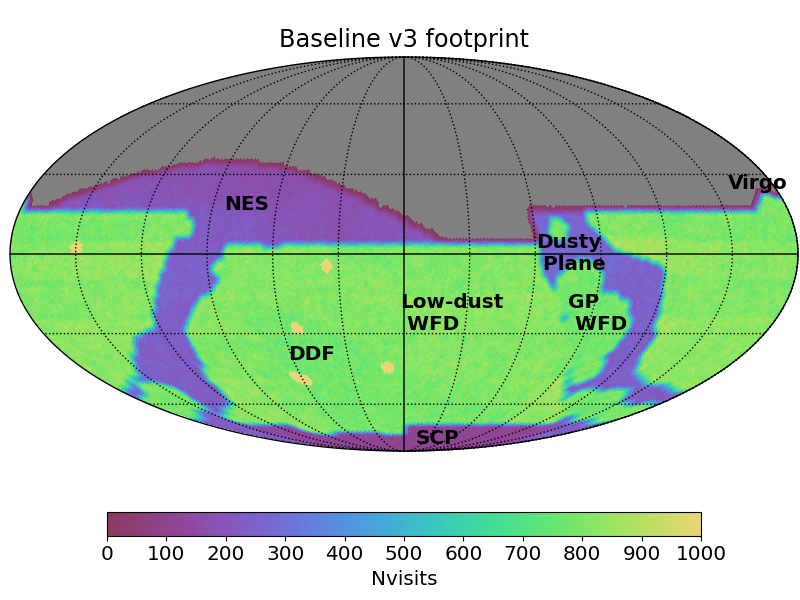
\includegraphics[width=4.7in]{figures/v3footprint.png}
    \caption{Number of visits per pointing in all filters for \texttt{baseline\_v3}. The color bar saturates at 1000. The Virgo cluster is visible on the right of the map, in the Northern hemisphere.%; the DDF fields have $\sim22,000$ visits per field. The Cosmos DDF has almost twice as many.
    }\label{fig:baselinev3Footprint}
\end{figure*}



\setlength\parindent{0.7cm}
\hangindent=0.7cm The footprint follows the description in section~\ref{q:Footprint} above, with the low-dust WFD ranging from a lower limit of Dec $\geq-70\degree$ ---or where the dust extinction exceeds $E(B-V)=0.2$--- to an upper limit of Dec $\leq+15\degree$ for 7~h $\lesssim$ RA $\lesssim$18~h and Dec $\leq+3\degree$ for 0 $\lesssim$ RA $\lesssim$ 7~h and 18~h $\lesssim$ RA $\lesssim$  24~h. The Virgo Cluster, centered on RA$=186.75\degree$, Dec$=12.171$\degree, with a radius of $8.75\degree$, is included in the low-dust WFD footprint. The NES ranges from the upper boundary of the low-dust WFD to $+10\degree$ ecliptic latitude. The SCP covers the remainder of the sphere below the WFD or Galactic Plane region. The Galactic Plane is covered in two parts; WFD-level regions near the Bulge and other regions of interest and a lower level of coverage in the remainder of the regions where dust extinction exceeds $E(B-V)=0.2$.  The median numbers of visits per pointing in these areas over the lifetime of the survey (in any filter) are: 795 visits per pointing in WFD-level areas (the low-dust WFD, Galactic Plane high coverage regions, the Magellanic Clouds, and Virgo cluster), 257 in the high dust extinction (low coverage) Galactic Plane regions, 195 in the NES, and 123 visits per pointing in the SCP. These are split between the $ugrizy$ filters with varying balances in different regions; the NES receives visits only in the $griz$ bands. The total number of visits per pointing is shown in \autoref{fig:baselinev3Footprint}. Evaluation of the footprint and distribution of visits within the Galactic Plane region will continue over the next year.

\hangindent=0.7cm Visits are acquired in $ugrizy$ filters, where $u$ band is available during periods where the lunar illumination is below 40\% and $z$ band is available during periods where the lunar illumination is above 40\% ($u$ and $z$ are swapped, the other filters remain in the camera at all times). Evaluation of this filter swapping procedure compared to alternative swapping strategies, for example alternating $z$ and $y$, will continue over the next year. 

\hangindent=0.7cm In the $u$ band, visits are acquired as a single exposure of 30 seconds to avoid becoming read noise limited; in $grizy$ bands, visits are acquired as a back-to-back set of two 15-second exposures. These 2x15s exposures are less efficient than a single 1x30s visit, due to additional shutter and readout time. During commissioning, 1x30s visits for all bands will be evaluated and, if viable, could be adopted; this would lead to an increase in efficiency of $\sim7\%$. 

\hangindent=0.7cm Visits are generally acquired in pairs separated by approximately 33 minutes. Visits to the same pointing within two hours of the first observation are suppressed at all times, which increases the number of visits that fall into other intervals  and typically pushes a third visit to the following night. Every seventh night, a third visit in the same filter as one of the original pairs is acquired within the same night at an interval of 2--7 hours (randomly assigned per night). These two factors together increase the number of return visits in the same filter during the period of two to 30 hours after the first visit.
Pairs of visits are acquired in different filters, with pairings driven by considerations on sensitivity to sky conditions and availability of filters on the filter wheel; $u$ is paired with $g$ or $r$ band, $g$ is paired with $u$ or $r$ band, $r$ is paired with $u$, $g$ or $i$ band, $i$ is paired with $r$ or $z$ band, $z$ is paired with $i$ or $y$ band, and $y$ is paired with $z$ or $y$ band. The SCOC may engage in further investigation of potential filter pairing strategies. 
\begin{figure*}[t!]
    \centering
    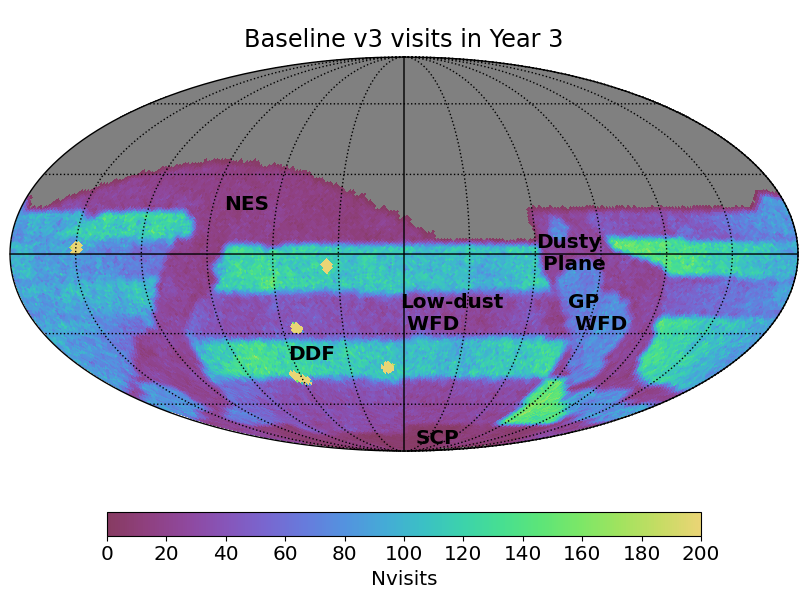
\includegraphics[width=2.5in]{figures/v3footprint_yr3.png}
    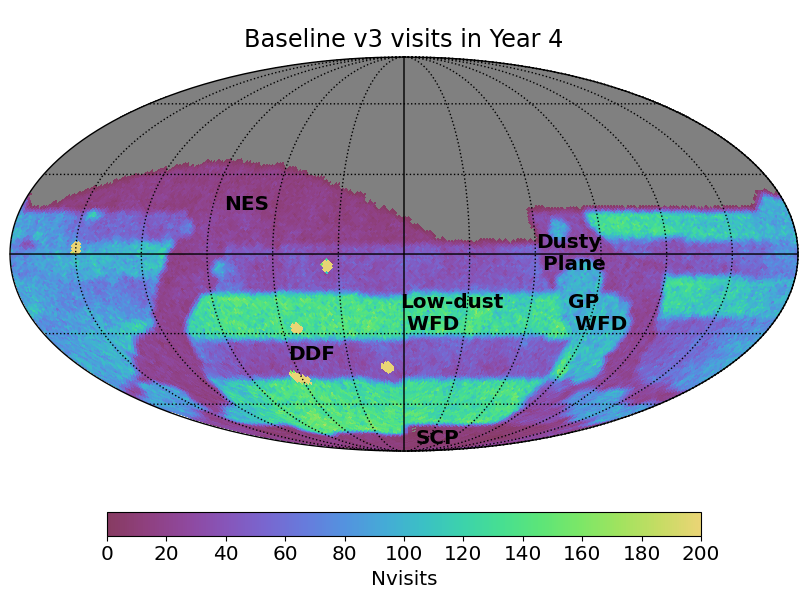
\includegraphics[width=2.5in]{figures/v3footprint_yr4.png}
    \caption{A half-sky rolling cadence is implemented in the low-dust WFD region. Half of the sky is ``active'' and observed at a higher intensity during its visibility season, while half of the sky is ``inactive'' and observed at a lower intensity during this same period. The left panel of this figure shows the visits  collected (in any filter) in (approximately) year 3 of the survey; the right panel shows the visits collected in (approximately) year 4. The central portion of the figure shows the declination bands clearly, as this part of the sky experiences only one observing season during the year selected so that it is strictly ``active'' or ``inactive'' depending on the year.  The outer edges of the low-dust WFD show a fuzzier boundary between the declination bands, as this part of the sky %(especially on the left-hand edge of the NES) 
    experiences both the end of an active season and the start of an inactive season (or vice versa) during this time period. This leads to a more uniform sky coverage. In this simulation, rolling cadence is only implemented in the low-dust WFD, and not the Galactic Plane, NES or SCP. The RA boundary where ``active'' and ``inactive'' declination bands swap after completing a full season is visible in the low-dust WFD region directly (below the ``GP WFD'' label). }\label{fig:baselinev3Rolling}
\end{figure*}

\hangindent=0.7cm A half-sky rolling cadence is implemented in the low-dust WFD, starting $\sim1.5$ years into the survey (when the first part of the sky which has had a complete season of observations in ``uniform'' cadence starts its second season). Four full seasons of rolling occur at each point in the sky, resulting in the last rolling season ending 0.5 years before the end of the survey. The sky is split into four declination bands, so that half of the sky (two bands) are ``active'' at any point in time during the rolling seasons; one of these bands is in the northern portion of the footprint and one in the southern portion, allowing distribution of follow-up requirements over a range of latitudes. An illustration of this rolling cadence, along with additional details, is provided in \autoref{fig:baselinev3Rolling}. The impact of this rolling cadence on the uniformity of the annual data releases will continue to be evaluated. 

\hangindent=0.7cm To generate a templates for the annual data releases, at least 3 to 5 images must be obtained in each bandpass each year on the WFD footprint. Yearly acquisition is desirable to avoid the impact of proper motion in template generation. This places a constraint on the minimum number of images per bandpass  acquired in any year, which is strongest in the $u$ band (as the $u$ band is only targeted to acquire about 50 images per pointing total, this results in $u$ band only minimally rolling; $g$ is only slightly above a similar threshold). 

\hangindent=0.7cm Good seeing visits (seeing $<0.8''$) in $g$, $r$, and $i$ bands are also prioritized in each year. This tends to distribute the best raw atmospheric seeing time into these bands relatively evenly. Due to wavelength-dependent effects on seeing, the resulting $g$ band delivered seeing is slightly worse than the delivered seeing in $r$ and $i$. A goal is set to obtain a minimum of three visits per pointing with delivered seeing $<0.8''$ in each of $gri$ bands.

\hangindent=0.7cm About 6.4\% of the total number of survey visits is devoted to the DDFs. The five DDFs are observed using pre-scheduled observations which are scheduled to ideally space themselves throughout the lunar cycle to optimize both cadence and depth (avoiding the brightest nights or times when the moon is up, for example). Observations for each DDF are acquired in sequences, which are defined as sets of 8 $u$, 10 $g$, 20 $r$, 20 $i$, 24 $z$, and 18 $y$ band 30 second visits (a single 1x30s visit in $u$, 2x15s exposures combined into a visit in $grizy$). As only 5 filters can be in the camera at one time, one of these bandpasses is always missing from the sequence; if the sequence is interrupted by weather or unexpected downtime, or the field becomes unavailable due to pointing constraints, the sequence will be cut short. Sequences that are interrupted or skipped are attempted on following days, but at a lower priority; missed sequences near the ends of seasons where the visibility windows on any night are shorter will tend to be skipped. The median number of visits per pointing for each of the DDFs is on the order of $10,000$, with the exception of the COSMOS field which receives almost $19,000$ visits. Following the recommendation in \autoref{q:DDF}, COSMOS is scheduled to achieve 10-year depth ($\sim10,000$ visits) by the end of year 3. It then continues to acquire observations at the same rate as the other DDF fields. The EDFS is split into two pointings; each pointing receives $\sim6,600$ visits. Generally, coadded DDF depths are about 1.3 magnitudes deeper in each bandpass than the coadded depth of a WFD pointing in the same bandpass. Dithering is implemented for each of the DDFs, with maximum offsets $\sim0.7\degree$ (the size of a raft). Optimization of the DDF scheduling is expected to continue through 2023.

\hangindent=0.7cm The near-sun twilight NEO microsurvey is implemented as recommended in \autoref{q:Micro}. Every fourth night during morning and evening twilight, visits are acquired in sets of four at low-solar elongations, separated by $\sim5$ minutes, with single exposure 15s visits in $r$, $i$, and $z$ bands. These visits are necessarily in high-airmass fields, which, as a side-effect, extends the season length for regions within this footprint (although with somewhat shallower visits). The NEO microsurvey footprint is shown in \autoref{fig:baselinev3Micro}.

\begin{figure*}[t!]
    \centering
    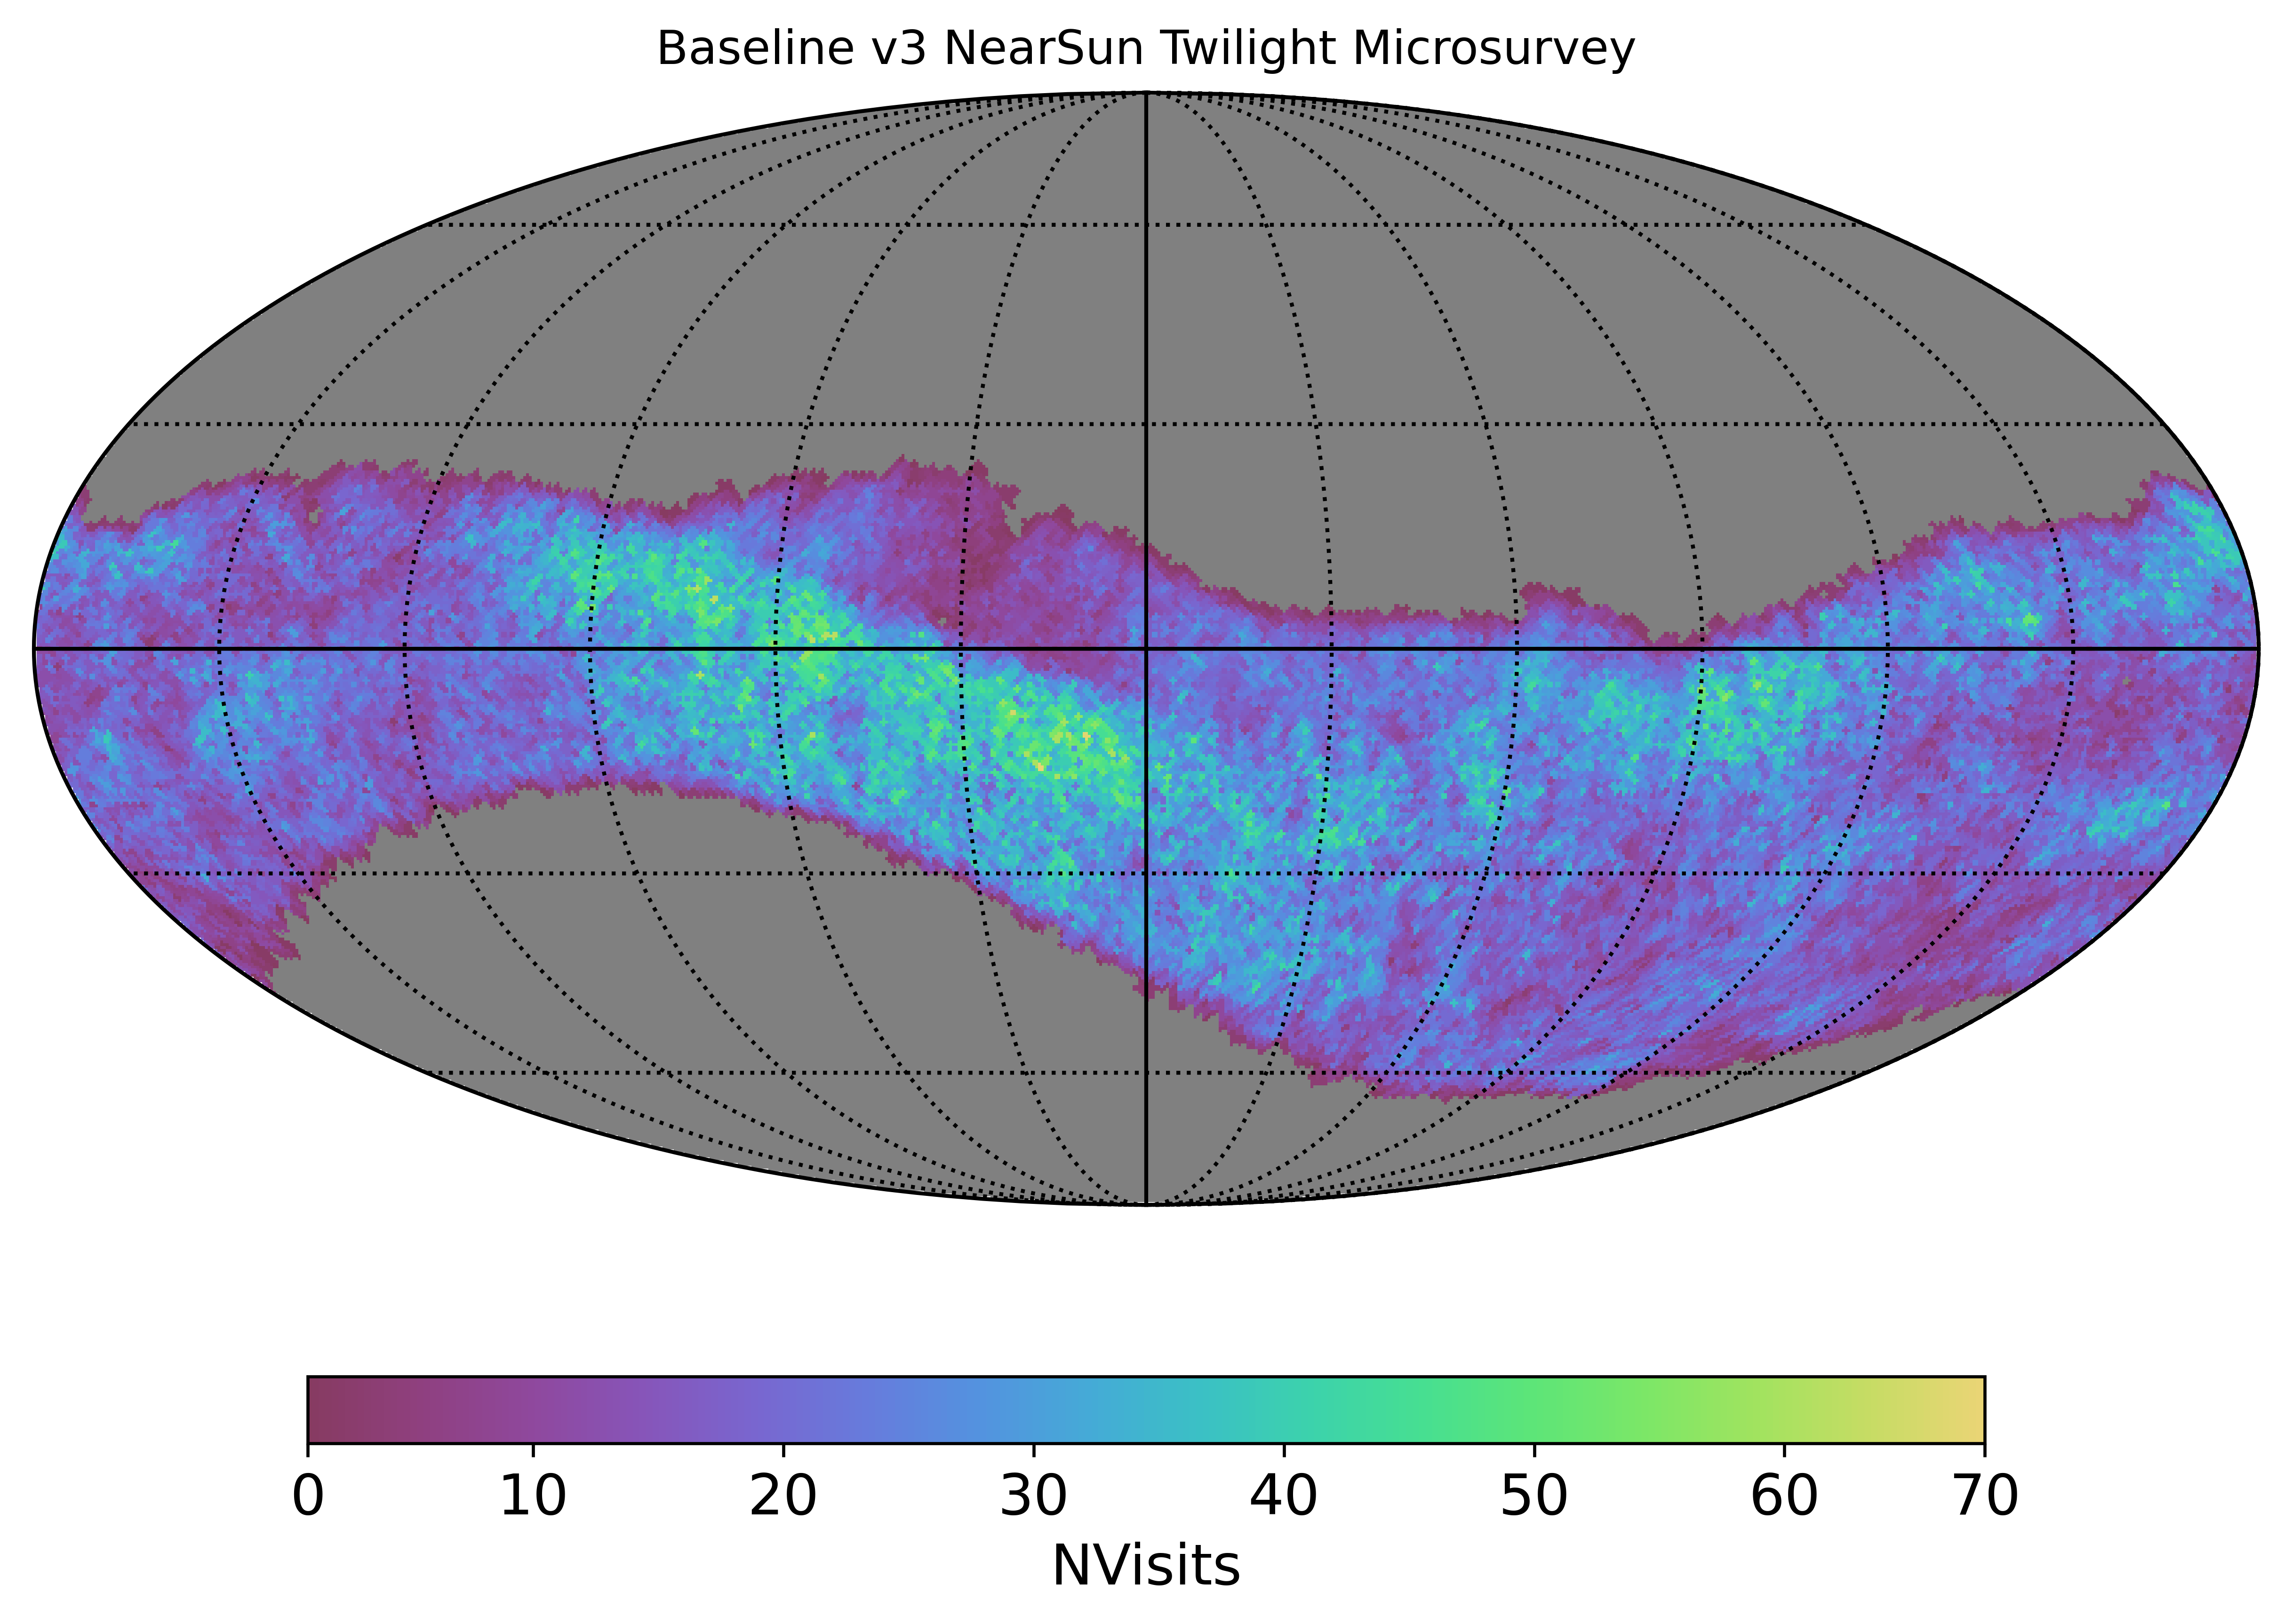
\includegraphics[width=4.7in]{figures/v3TwilightMicrosurvey.png}
    \caption{The footprint of the near-sun NEO twilight microsurvey. This microsurvey executes every fourth night in morning and evening twilight, with a footprint defined by solar elongation with $<=60\degree$ and airmass $X<=2$ limits, and regions with Dec $<= 30\degree$ and ecliptic latitude $< 40\degree$. Within the twilight period, four 15s visits separated by about five minutes are attempted. These areas of the sky are only visible for a short period; linking within a given night aids the discovery of near-sun asteroids. }\label{fig:baselinev3Micro}
\end{figure*}
\clearpage

\section{Compendium of points open for further exploration and refinement.}
The topics that the SCOC should focus on in the next round of deliberations follow.

\begin{itemize}

\item The SCOC recommends that the investigation of the filter swapping schemes on the filter wheel continue. After the November 2022 workshop a few experiments in swapping $u$,$z$, and $y$ instead of $u$ and $z$ were implemented in \texttt{v2.99} simulations. More work is needed to understand the impacts of this decision on the DDFs as well as on the WFD. Filter pairing prescriptions for the observation pairs should also be explored in some more depth.

\item The current SCOC recommendation is to implement a rolling cadence with a half-sky rolling scheme and a 0.9 rolling weight. However, rolling impacts the uniformity of static data releases which, as experts in the community have highlighted, is necessary for static sky science in general and cosmology in particular. This issue may be resolved or mitigated at the software level in the creation of coadds and catalogs, rather than at the scheduler level. The community should specify the desired and necessary requirements for uniformity to enable the exploration of data processing solutions to this problem. Depending on the feasibility of a solution to ensure sufficient uniformity, the SCOC recommendation on rolling may be re-evaluated. 

\item The SCOC is not ready to finalize a recommendation for the
filter balance in the Galactic Plane, or for a final Galactic Plane/Bulge footprint, or the rolling scheme to be implemented on the Galactic Plane. The SCOC will work with the SMWLV and TVS SCs to ascertain the best solutions for Galactic science on filter balance and footprint. These decisions should, however, not impact decisions relating to the WFD and the time spent collectively on Galactic regions should not change.
Galactic Plane pencil-beam surveys need to be defined more clearly to assess if they would ultimately result in ``nano-surveys'', which will require a fraction of time too small to be optimized at this stage, or to evaluate the possibility of incorporating them in a final Galactic Footprint recommendation.

\item While the SCOC recommends the filter balance as implemented starting in \texttt{baseline\v2.0} should not be changed, it is possible that rebalancing the
exposure time to compensate for performance and throughput in some filters as compared to others or shortening exposures in filters where the throughput exceeds expectations enabling the collection of more images in that filter (or overall) would lead to
enhanced LSST science. The SCOC cannot finalize this recommendation at this time due to
missing information about the characteristics of the system-as-built.



\item {The SCOC will continue working in 2023 with the community to identify the specific intra-night cadence that maximizes the science throughput of the DDF survey, while not impacting the science performed by other surveys.} 

\item{The SCOC shall work in coordination not only with the scientific community but also with the leadership of Rubin and the Euclid mission to identify cadence requirements, co-observing strategies, and paths to produce the data products that will enhance science through the coordinated observing of the EDFS.}

\item The SCOC recommends the decisions on the ToO strategy be based on a recommendation to be delivered by science experts and Rubin experts in  2023 in a dedicated workshop.

\item The SCOC awaits commissioning assessments of the viability of collecting images in a single 1x30s exposure in all filters (rather than 2x15s), which would lead to an increase in efficiency. The SCOC has thus far seen favorably a potential switch to a single 1x30s exposure and the associated efficiency gain. If commissioning reveals that a 1x30s exposure is indeed technically viable, the SCOC should review the benefits (and potential drawbacks) of visits in a single exposure and, if adopted, reassess its recommendations in the light of this increased efficiency.


\item The SCOC recommends implementing a detailed coordination plan with the Early Science Rubin team to reach a final recommendation on the strategy to be implemented in the first year of the survey, including a scheme for the construction of templates.


\end{itemize}

\label{sec:refinements}
\clearpage

% You can also use the \input command to include several content files.



